\chapter{模式构架}\label{模式构架}
%\addcontentsline{toc}{chapter}{模式结构}
\echapter{Model Architecture}

\section{网格构建}\label{网格构建}
\esection{Mesh Construction}
\begin{mymdframed}{代码}
  本节对应的网格类型可在\texttt{/include/define.h}中进行选择。
\end{mymdframed}

通用陆面模式(CoLM,the Common Land Model)首先对陆地表面进行剖分,将模拟区域按一定规则划分成单元(Element),模拟分辨率决定了单元平均面积的大小。CoLM中包含三种单元划分规则:1)经纬度网格(图~\ref{fig:经纬度网格});2)非结构网格(三角形/六边形)(图~\ref{fig:六边形单元网格},~\ref{fig:三角形单元网格});3)流域单元(Catchment)(图~\ref{fig:流域单元网格})。除以上三种网格外,CoLM实际可使用任意形状单元的网格。

{
  \begin{figure}[htbp]
    \centering
    \includegraphics[width=0.8\textwidth]{Figures/模式构架/网格-格点.jpg}
    \caption{CoLM中可使用的网格(1):经纬度单元}
    \label{fig:经纬度网格}
  \end{figure}
}
{
  \begin{figure}[htbp]
    \centering
    \includegraphics[width=0.8\textwidth]{Figures/模式构架/网格-六边形.jpg}
    \caption{CoLM中可使用的网格(2):六边形单元}
    \label{fig:六边形单元网格}
  \end{figure}
}
{
  \begin{figure}[htbp]
    \centering
    \includegraphics[width=0.8\textwidth]{Figures/模式构架/网格-三角形.jpg}
    \caption{CoLM中可使用的网格(3):三角形单元}
    \label{fig:三角形单元网格}
  \end{figure}
}
{
  \begin{figure}[htbp]
    \centering
    \includegraphics[width=0.8\textwidth]{Figures/模式构架/网格-流域.jpg}
    \caption{CoLM中可使用的网格(4):流域单元网格}
    \label{fig:流域单元网格}
  \end{figure}
}

\subsection{经纬度网格}\label{经纬度网格}
\esubsection{Regular Latitude-Longitude Grids}
经纬度网格通过规定经度和纬度分割线的位置来建立,单元的边界由东西两段经线和南北两段纬线组成。经纬度网格的分辨率通常使用经纬度分割线的间距来表达,例如,分辨率为0.5\textdegree 表示相邻两条纬度分割线和经度分割线的距离均为0.5\textdegree。经度分割线和纬度分割线分别可以是不等间距的,当间距不等时,需从外部数据读入分割线的位置来定义模拟区域的经纬度网格。

\subsection{非结构网格}\label{非结构网格}
\esubsection{Unstructured Grids}
在原有的经纬度网格基础上,CoLM 新开发了一个非结构化网格构建工具,它可以基于多个水平分布特征,自动识别不同区域所需的网格分辨率,生成包括三角形网格和多边形网格(以六边形网格为主)在内的无规则拓扑关系网格。具体而言,非结构网格的分辨率取决于所指定的一个或者多个目标的分布特征(例如高程、坡度、土地利用、植被类型等)。该工具可在目标变化梯度较大的地区采用高分辨率,在变化梯度较小的地区采用低分辨率。因此基于非结构化网格的多分辨率模拟保留了全局模型的整体结构,同时支持局部区域的高分辨率模拟。

在非结构网格的构建过程中,该工具首先基于 Delaunay 三角网等值线生成算法构建初始网格,即将经纬度网格数据转化插值,生成铺盖整个球面的三角形网格数据;接着根据所选取的目标进行一次或者多次细化与网格结构调整;再依次连接具有相同顶点的五至七个三角形重心生成多边形网格,最后输出全球区域的三角形或多边形可变分辨率网格。总之,非结构网格具有灵活性强、节点和单元的分布可控性好、能较好地控制网格的大小和节点的密度等优点。模式运行流程如图~\ref{fig:非结构化网格CoLM总体运行流程图} 所示。

{
  \begin{figure}[htbp]
    \centering
    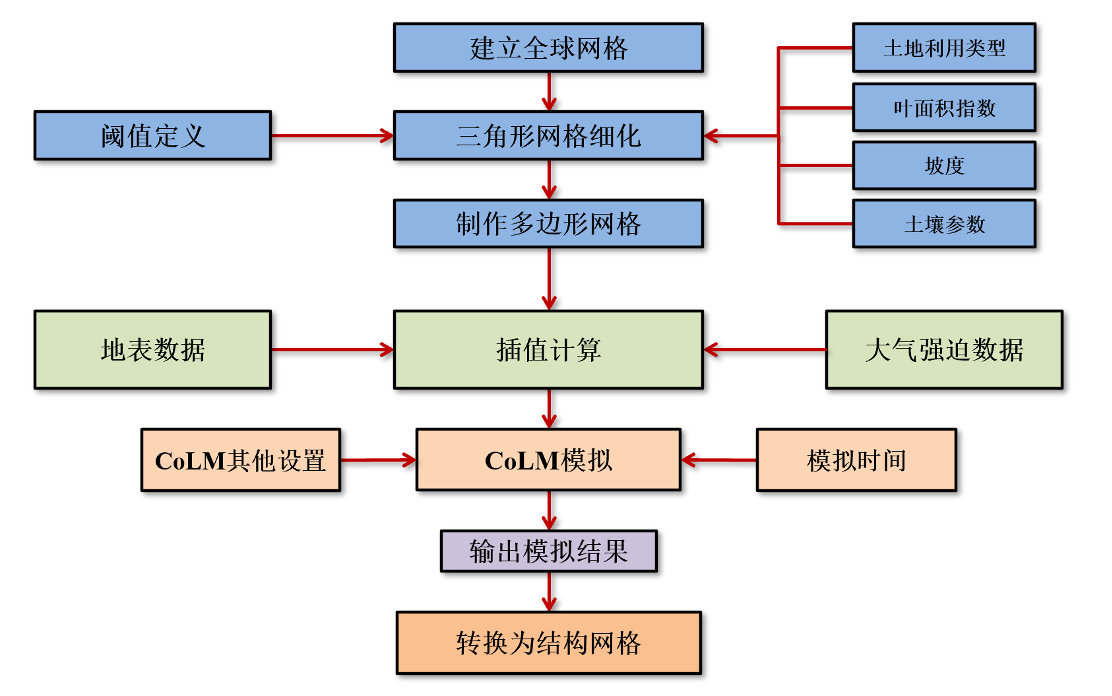
\includegraphics[width=0.8\textwidth]{Figures/模式构架/非结构化网格CoLM总体运行流程图.png}
    \caption{非结构化网格CoLM总体运行流程图}
    \label{fig:非结构化网格CoLM总体运行流程图}
  \end{figure}
}

该工具基于非结构化一致性三角-六边形构建算法 \citep{fatichi2020soil,walko2008ocean,walko_direct_2011},以准均匀的全局三角形(Delaunay)的网格化方法为理论依据。其中非结构网格构造流程如图~\ref{fig:非结构化网格生成流程图} 所示,具体介绍如下:
{
  \begin{figure}[htbp]
    \centering
    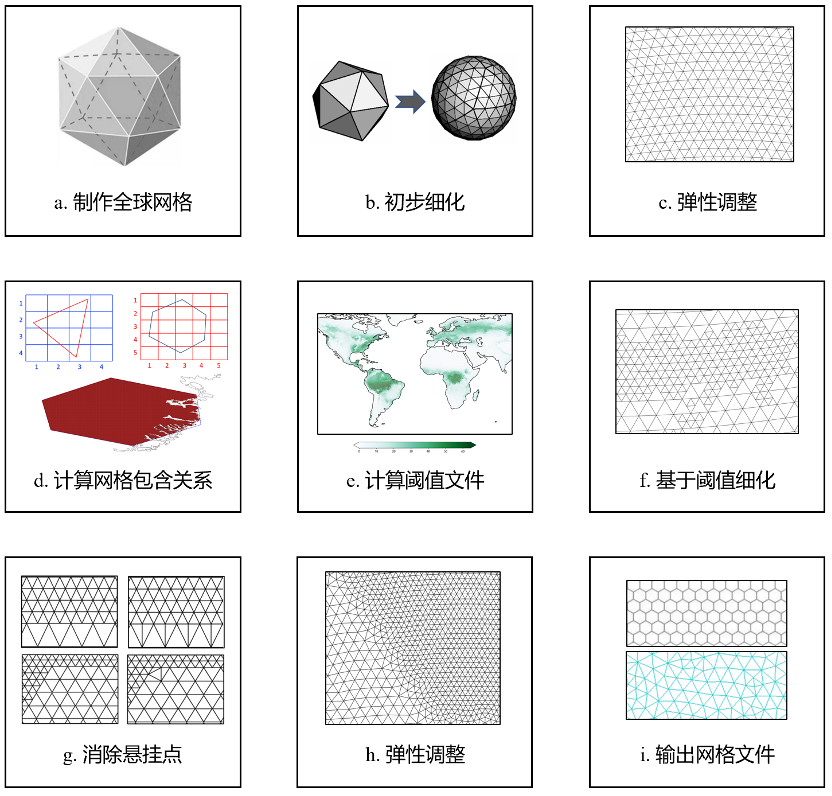
\includegraphics[width=\textwidth]{Figures/模式构架/非结构化网格生成流程图.png}
    \caption{非结构化网格生成流程图}
    \label{fig:非结构化网格生成流程图}
  \end{figure}
}

{
  \begin{table}[htbp]
    \centering
    \caption{细化阈值文件}
    \label{tab:细化阈值文件}
    \begin{tabular}{@{}ll@{}}
      \toprule
      变量名                       & 具体描述                     \\ \midrule
      ${\rm LCT}_{\rm number}$     & 网格包含的土地类型数量       \\
      ${\rm LCT}_{\rm dominant}$   & 网格主导土地类型             \\
      ${\rm iter}_{\rm max}$       & 三角形网格最大细化迭代次数   \\
      LAI                          & 叶面积指数                   \\
      slope                        & 坡度                         \\
      $K_{\rm sat}$                & 饱和导水率                   \\
      $k_{\rm s}$                  & 土壤固体导热系数             \\
      $k_{\rm dry}$                & 土壤导热系数(干燥)         \\
      $k_{\rm sat,frz}$            & 土壤导热系数(冻结、饱和)   \\
      $k_{\rm sat}$                & 土壤导热系数(未冻结、饱和) \\ \bottomrule
    \end{tabular}
  \end{table}
}

{
  \begin{figure}[htbp]
    \centering
    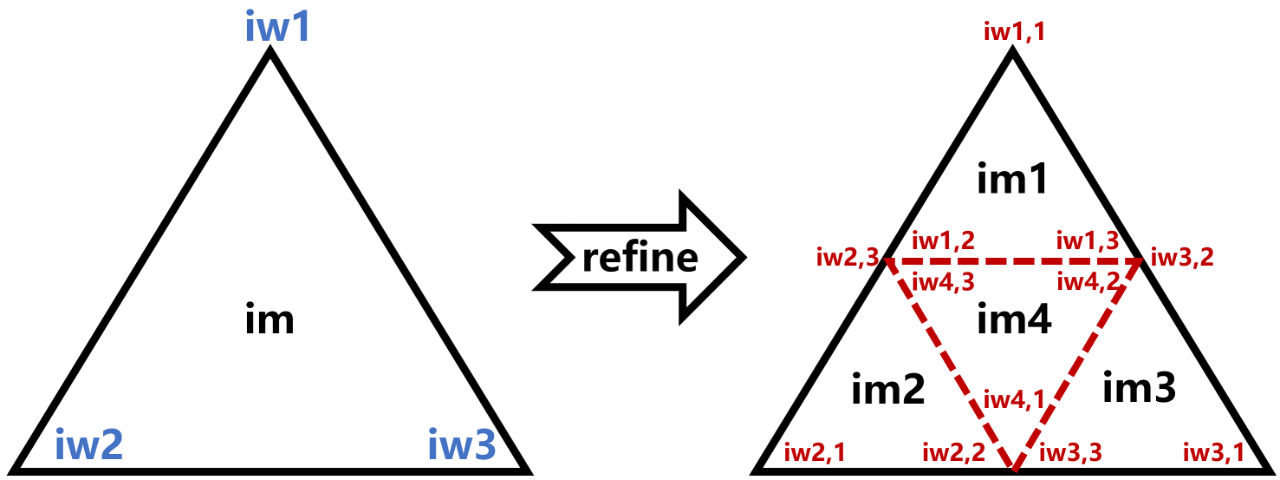
\includegraphics[width=\textwidth]{Figures/模式构架/三角形网格简易细化.png}
    \caption{三角形网格简易细化,其中iw为三角网格的顶点,iv为三角网格各边的中点,im为三角网格的重心。}
    \label{fig:三角形网格简易细化}
  \end{figure}
}

\begin{enumerate}
  \item 构建初始网格

    在此过程中,首先将一个正二十面体投射到地球表面,它的12个顶点中有两个位于南北两极,其余的位于$\pm\arctan(1/2)$ 纬度。正二十面体网格的二维投影基于0\textdegree 经线所在经线圈与与0\textdegree 维度所在纬线圈轴对称。这有利于在计算包含关系时简化运算步骤。同时每个区域被划分为面积基本相同大小的三角形分块,以满足非结构网格初步细化和提升并行化计算效率的需要。

  \item 初步细化

    在此步骤中,网格生成工具能够将每个球面三角形面细分为NXP $\times$ NXP更小的三角形,其中NXP可设置为任意正整数,代表所选的网格分辨率。NXP定义为两个相邻多边形网格的水平网格间距(网格单元面积的平方根),网格的分辨率大约等于7200公里/NXP。因此,如果试图在网格上获得100公里的水平网格间距,应将NXP设置为“72”。这种网格配置采用基于二十面体改进的六边形或三角形网格单元的非结构化网格,从而避免了传统经纬度网格的南北极奇点。该网格配置为局部网格细化提供了一种完全无缝的自然适应性,不需要额外特殊的网格嵌套算法。

  \item 弹簧动态调整

    考虑到地球球面对三角形网格实际边长的影响,通过初步细化生成的三角形并不等同于等边三角形。\citet{tomita2002optimization}描述了一种称为“Spring Dynamics”的计算方法,用于在准均匀的全局网格上调整三角形网格单元的形状和大小。该方法代表了一种物理模拟,其中网格中的每个边都像弹簧一样在其顶点间施加吸引力或相反的力,该弹力取决于其自身的长度、平衡长度和弹簧系数。该研究表明,将平衡长度设置为使弹簧松弛在数值上稳定的最大可能值,即接近整个网格的平均边长,会产生最小的网格单元尺寸的空间变化,并且调整过程能显著提高模型的数值精度。

  \item 计算包含关系

    CoLM非结构网格的空间细分基于三角形网格与阈值数据(部分地表数据,如表~\ref{tab:细化阈值文件})进行。一般来说,三角形网格的分辨率远低于阈值数据集。这些高分辨率网格(以下简称像素)构成了非结构化网格。在进行网格细化之前,需要计算两者间的包含关系,并得到每个网格对应像素的索引,以便识别像素对非结构网格的归属。最后,根据这些像素的信息,用户可以了解特定网格内的空间异质性,并决定是否需要对其进行细化。这个过程将在细化过程中的每次迭代中执行。

  \item 阈值文件计算


    \citet{walko_direct_2011} 中的细化面积和程度是通过分配一系列点的经纬度坐标来确定的(例如,(lat = 30.1, lon = 120.5); \dots)加上影响半径(例如,(R = 1km); \dots)。与之不同,CoLM的网格细化工具能够根据各种指标确定精细化的区域。关于这些指标的详细信息可以在表~\ref{tab:细化阈值文件} 中找到。该工具允许对一个或多个网格进行细化,并约束到用户定义的阈值。换言之,CoLM 可以根据任意数量的重要特征对网格进行细化,例如 ${\rm LAI}$ 的标准差,网格内土地利用类型数量等。图~\ref{fig:多阈值非结构网格细化} 展示了基于多种不同地表特征进行细化得到的全球陆面多边形网格。

    {
      \begin{figure}[htbp]
        \centering
        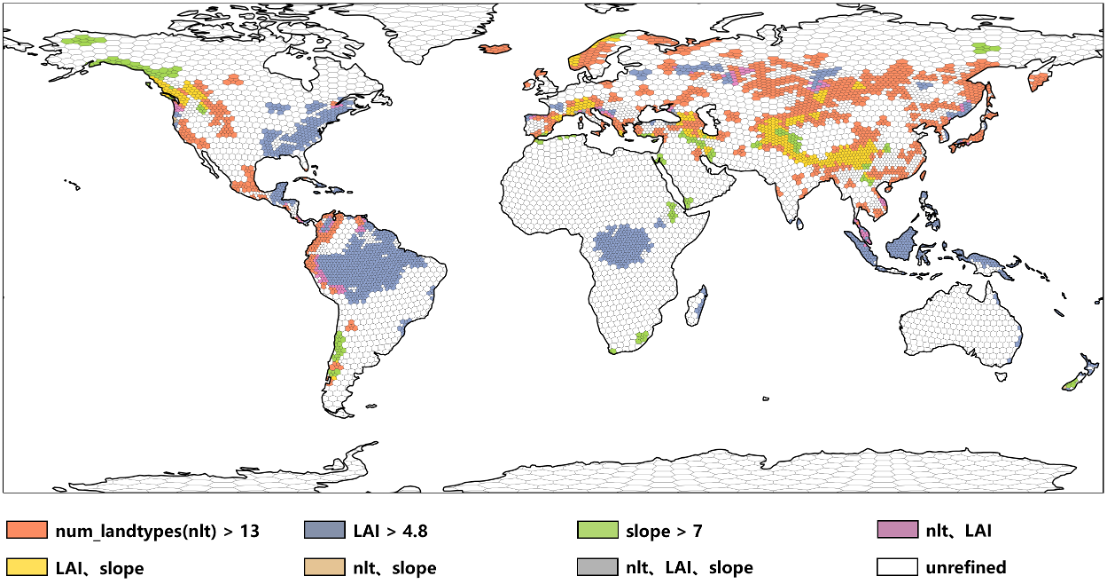
\includegraphics[width=\textwidth]{Figures/模式构架/多阈值非结构网格细化.png}
        \caption{多阈值非结构网格细化示例。其中num\_landtypes(nlt)代表基于土地利用类型的数量阈值细化的网格,LAI代表基于叶面积指数阈值细化的网格,slope代表基于坡度阈值细化的网格,undfined代表不满足上述细化阈值的网格,nlt,LAI代表同时满足基于土地利用类型的数量阈值和基于叶面积指数阈值细化的网格(依此类推)。}
        \label{fig:多阈值非结构网格细化}
      \end{figure}
    }

  \item 阈值细化

    如图~\ref{fig:非结构化网格生成流程图} 所示,本步骤主要实现三角形网格的阈值细化。利用生成的初始三角形网格包含关系,可计算三角形网格下各阈值数组,再根据阈值标记网格是否需要细化。如图~\ref{fig:三角形网格简易细化} 所示,通过将三角形网格“分成四格”,即可提高三角形网格的分辨率。然后,将新生成的网格信息添加到原始数组中,并标记被细化的网格。在计算新生成网格的包含关系时,只需要遍历被细化三角形最小外围矩形内的经纬度网格,可以大大减少计算时间。当迭代次数超过阈值或所有三角形网格满足阈值时,阈值细化终止,程序将输出最终生成的带有包含信息的三角形网格信息数据(见表~\ref{tab:细化阈值文件})。图~\ref{fig:根据LAI对非结构网格进行多重细化} 展示了基于叶面积指数特征进行多层级细化所生成的多边形网格结构。

    {
      \begin{figure}[htbp]
        \centering
        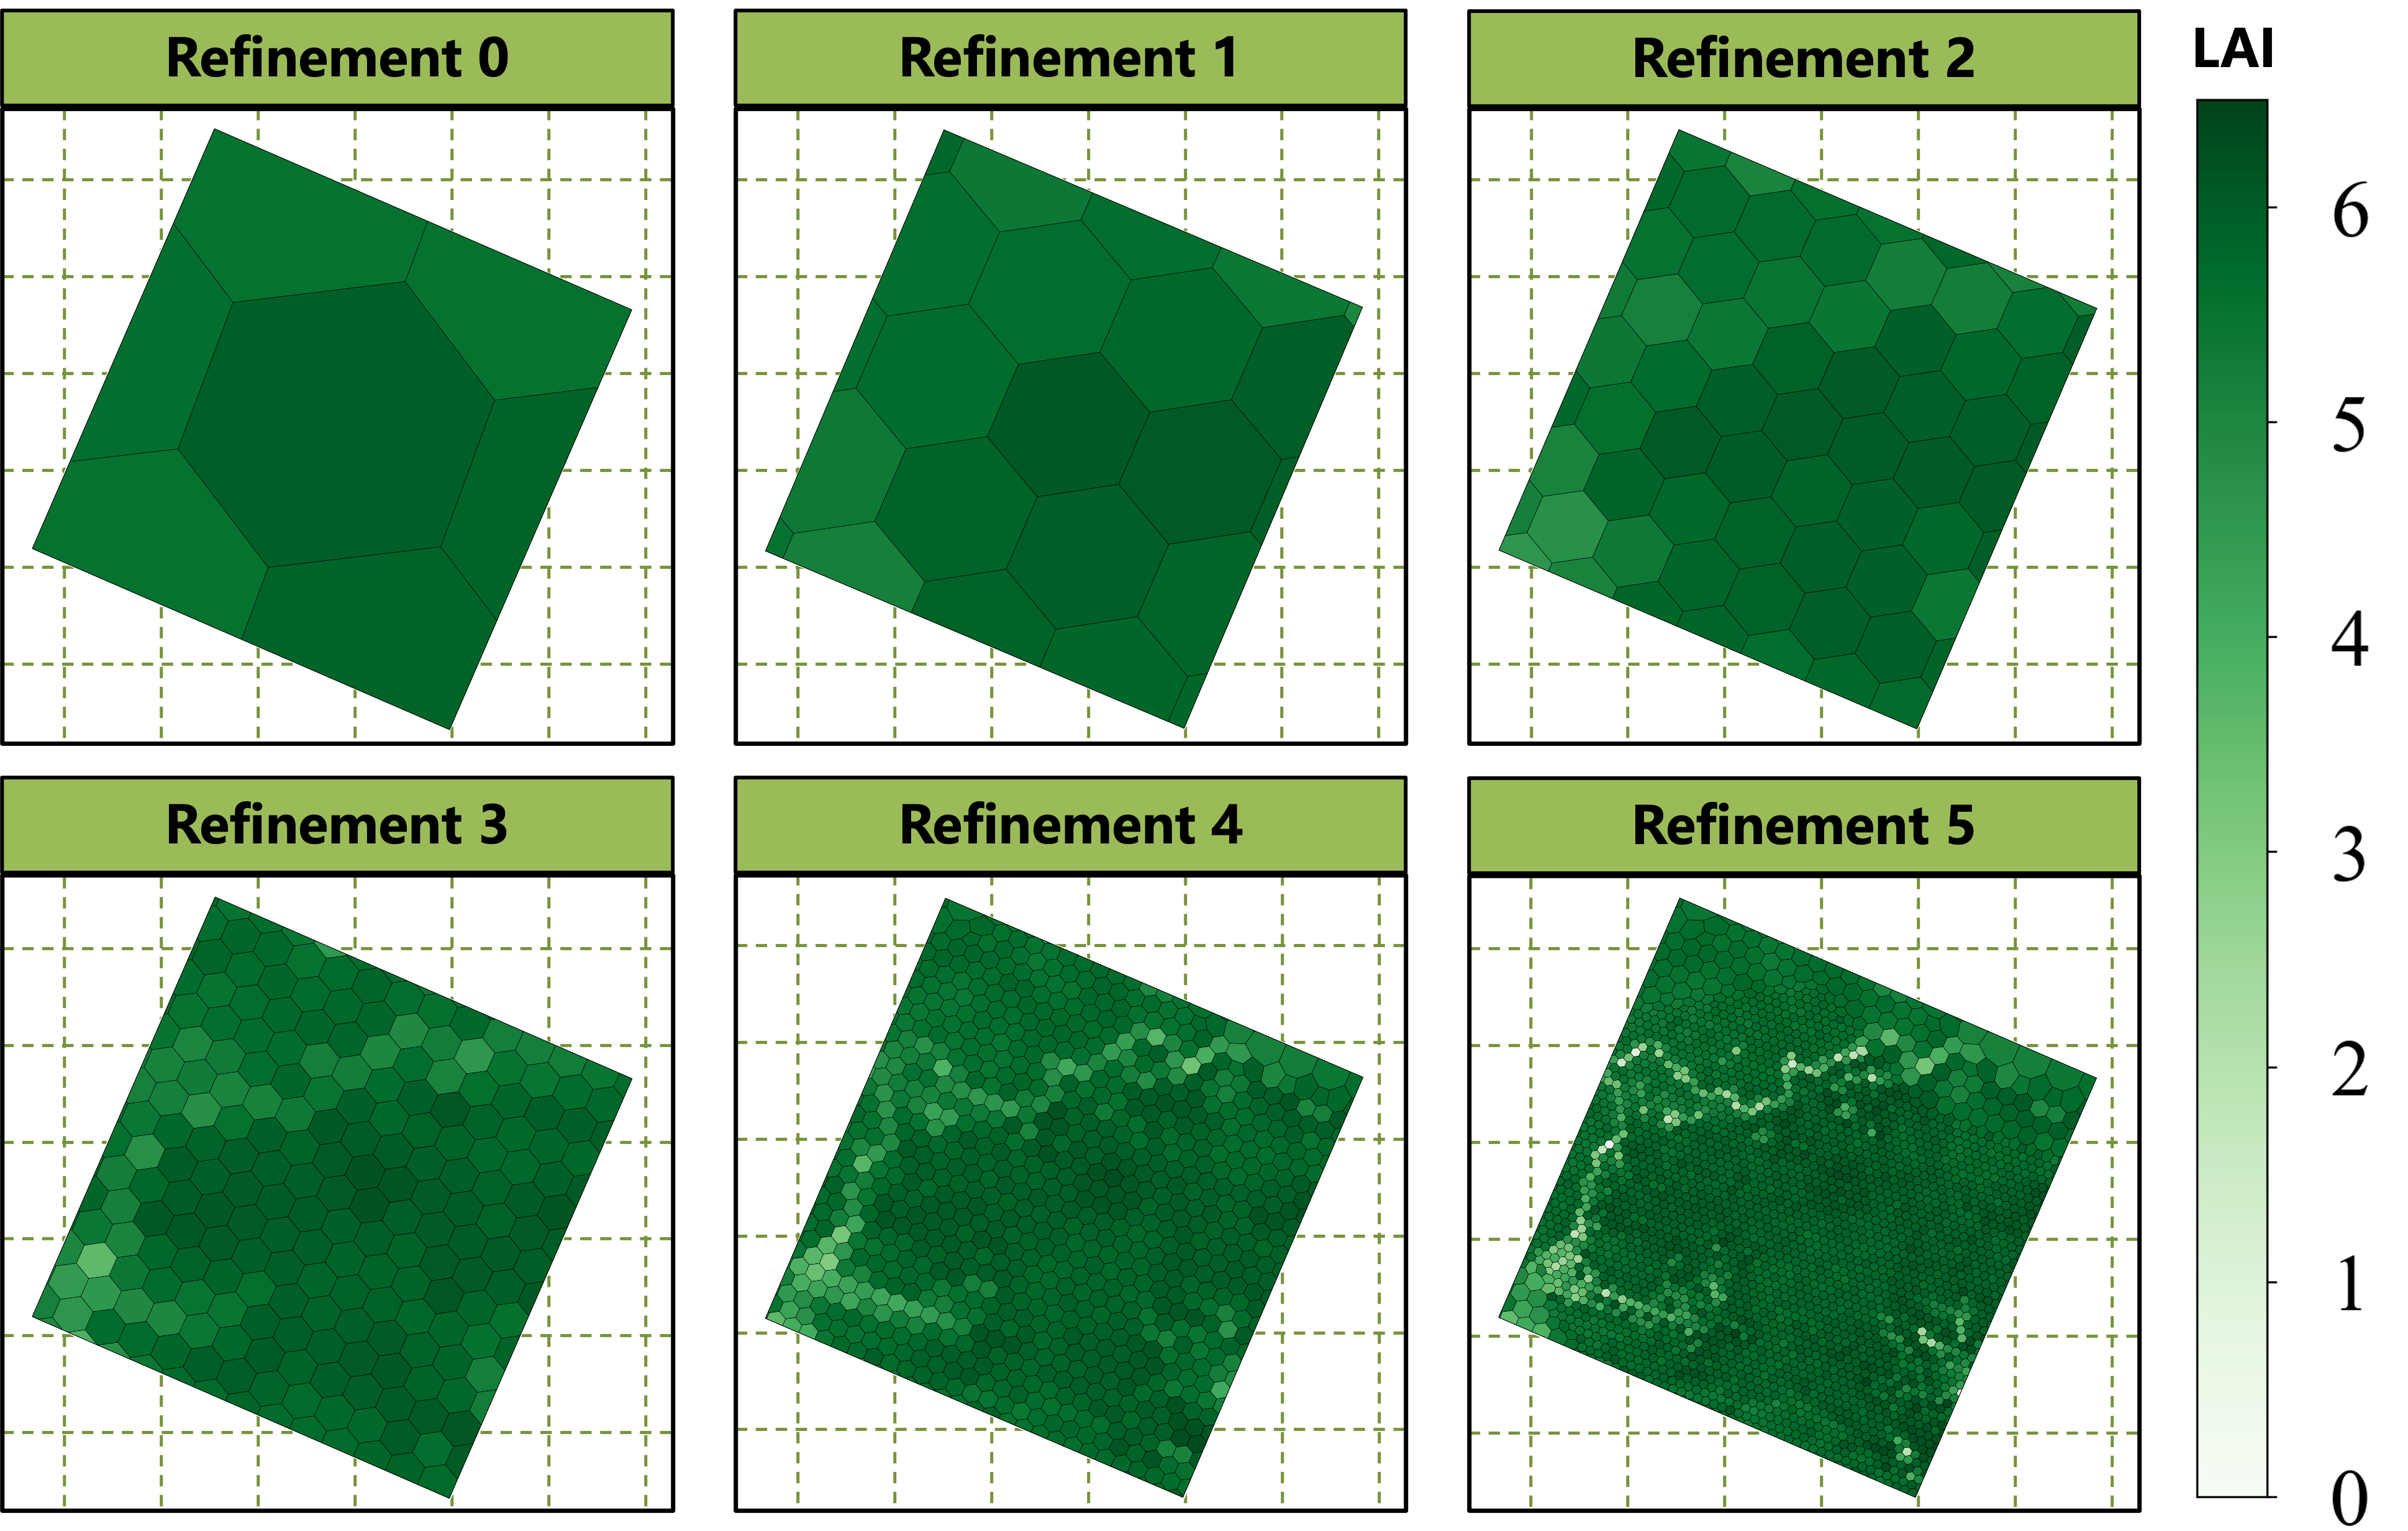
\includegraphics[width=0.8\textwidth]{Figures/模式构架/根据LAI对非结构网格进行多重细化.png}
        \caption{根据LAI对非结构网格进行多重细化}
        \label{fig:根据LAI对非结构网格进行多重细化}
      \end{figure}
    }

  \item 清除悬挂点\\
    该步骤将网格细化生成的附着在原始三角形边缘上的点称为悬挂点。为了保证每个三角形只与三个相邻三角形共享边,我们针对两种情况设置了不同的悬挂点消除方案。如图~\ref{fig:非结构化网格生成流程图} 顶部所示,对于细化边缘较平坦的区域,可以连接悬挂点与其相邻三角形的顶点。而对于一些凹陷区域,如图~\ref{fig:非结构化网格生成流程图} 底部所示,由于多个悬挂点位置相邻,直接连接悬挂点与其相邻三角形的顶点会使顶点被相邻的八条边共享,导致生成多边形网格时产生八边形,因此我们采用了特殊的细化方法来避免这一问题。此外,在消除悬挂点时,如果两个细化区域的边界相遇,也容易产生八边形。综上所述,在消除悬挂点前,需要对初步细化后的网格进行如下预处理:
    \begin{enumerate}
      \item 遍历所有未细化的三角网格。当其相邻的3个三角形网格中有1个以上被细化时,该三角形网格需要被细化。
      \item 在三角形网格中找到并记录凹陷区域(即图~\ref{fig:非结构化网格生成流程图} 底部细化区域)。当两个凹陷区域有一个公共三角形网格时,细化组成它们的三个三角形网格
      \item 循环遍历所有三角形网格顶点,计算剔除悬挂点后该点将添加的邻边数,当增加后其邻边数大于七时,细化其所有邻接三角形网格。在预处理过程中,三个进程依次进入迭代。当三个过程同时没有进行网格细化时,视为预处理完成。预处理完成后,可以进行消除悬挂点操作(即图~\ref{fig:非结构化网格生成流程图}),并得到可用于构建多边形网格的三角形网格。
    \end{enumerate}
  \item 网格调整和多边形网格生成\\
    在消除悬挂点的操作过程中,消除凹陷区域会生成许多钝角三角形。而多边形网格由三角形网格重心连接而成,因此过多的钝角三角形会导致生成的部分多边形与正多边形偏差较大,进而降低网格的各向同性,最终影响网格在CoLM等水文模型中的应用。为了在不过度影响原有网格结构的情况下对网格进行校正,本文根据钝角三角形角度与边长计算经纬度位移分量,并对其进行迭代调整。当不存在钝角三角形或迭代次数超过阈值时,调整结束。在每次迭代过程中,通过三角形网格重心构造多边形网格,并计算三角形网格与正三角形、多边形网格与正多边形角度的标准差,这是衡量非结构网格自身各向同性的标准之一。在每次迭代过程中,通过三角网格的重心构造多边形网格,并计算三角形网格与正三角形、多边形网格与正多边形的标准差,这是衡量网格自身物理结构质量的标准之一。迭代完成后,通过三角网格重心所构造处的最后一个多边形网格即为最终结果。
  \item 输出网格文件\\
    在上述步骤完成之后,可输出两种类型的网格。一是最后一次迭代生成的三角形网格,二是根据前者重心连接构造的多边形网格。在 MPI 版本中,无需将地表、大气等初始数据的存储方式由经纬度网格转换为非结构化网格,就可以实现 CoLM 中地表水文过程在非结构化网格上的模拟。
\end{enumerate}


\subsection{流域单元网格}\label{流域单元网格}
\esubsection{Catchment‐based Grids}
流域单元为面积大致相同的集水区域(图~\ref{fig:流域单元网格})。流域单元考虑了网格单元之间的水文关联以及单元内部的水文结构,基于流域单元网格,可建立对产流和汇流动力学过程的模拟方案。此外,流域单元及其次级单元(高度带单元)的划分主要依赖高程数据,在陆面过程受地形影响较为显著的区域,采用流域单元网格可显著减少网格内陆表变量的异质性,提高模式模拟的精度。

CoLM中的流域单元网格为三级结构:第一级为流域单元,第二级为高度带单元,第三级为次网格单元(图~\ref{fig:流域单元示意图})。其中,流域单元和高度带单元使用水文学数据生成,次网格单元的生成方法与其他网格中的次网格单元相同(见~\ref{次网格}~节)。

{
  \begin{figure}[htbp]
    \centering
    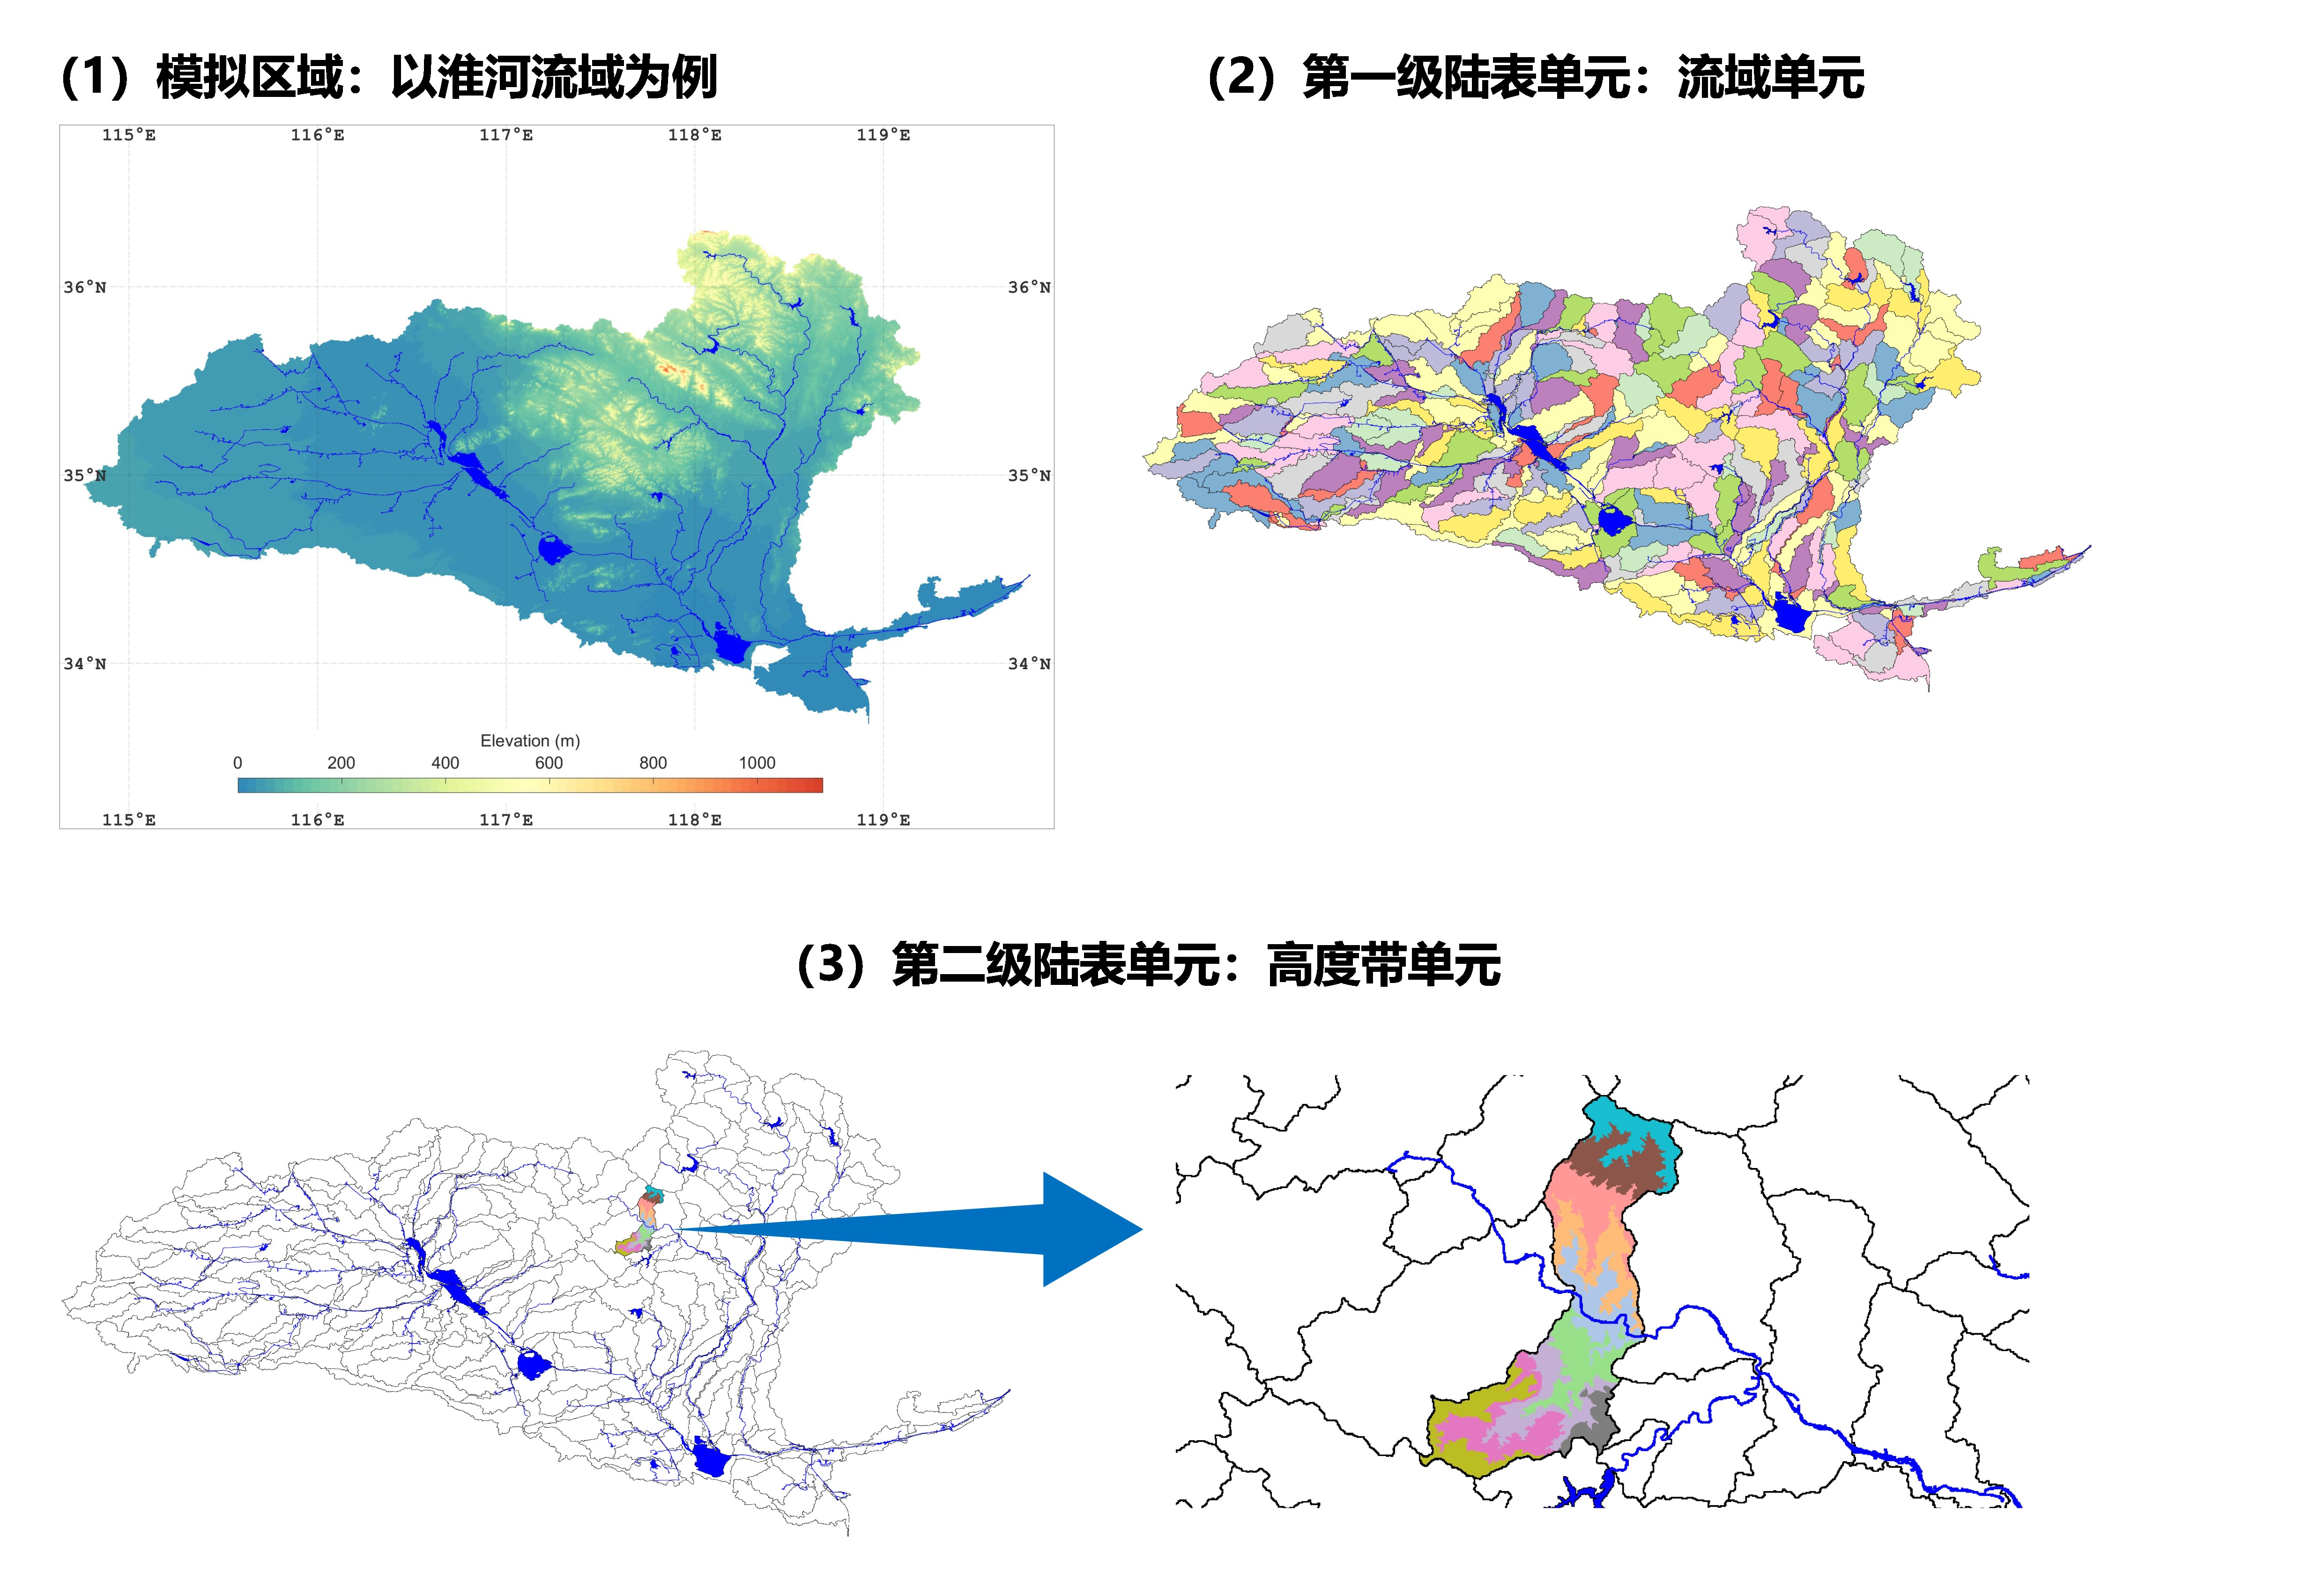
\includegraphics[width=\textwidth]{Figures/模式构架/流域单元示意图.jpg}
    \caption{CoLM中的流域单元网格划分示意图}
    \label{fig:流域单元示意图}
  \end{figure}
}

流域单元(第一级)为面积大致相同的集水区域(图~\ref{fig:流域单元示意图}(2))。流域单元网格的分辨率表示为一个单元的面积阈值(即河道集水区域的面积阈值,记为Cat-size)。流域单元的划分使用高分辨率的“上游集水面积”(UPA)和“水流方向”格点数据(其中的格点以下称为像素点),分为两个步骤。
第一步,提取研究区域的河道像素点并将其分段。此处的河道像素点定义为上游集水面积大于或等于Cat-size的像素点,未必为真实的河道。提取完成后,根据以下三个规则从下游至上游将河道分段:1.一段河道内没有河道分支;2.局部集水面积(定义为该河段的总集水面积减去上游河道的集水面积)不超过Cat-size;3.河道长度小于Cat-size的平方根。其中,规则1的目的是排除汇流点在流域单元内部的情况,以更合理地进行汇流过程的模拟;规则3的目的是避免流域单元较为狭长,以减少单元内部陆表变量的变化。
第二步,根据河道分段将研究区域划分为流域单元。一个流域单元定义为一段河道的局部集水区域。对每个像素点,可根据水流方向数据向下找到其所在的流域单元。

高度带单元(第二级)为主要依赖高程进行划分的流域单元内部子区域(图~\ref{fig:流域单元示意图}(3))。因流域面积较大时,一段河道的上下游会有落差,CoLM中不直接使用高程数据对流域单元进行划分,而是使用像素点的排水高度。排水高度定义为一个像素点和它流入的河道点的高度差(Height above nearest drainage, HAND),可根据高程数据和像素点与河道的汇流关系计算得出。此外,为了基于高度带单元进行产流动力学过程的模拟,CoLM对高度带单元的划分进行了进一步的约束,划分后的高度带单元需满足:1)连通性;2)每个高度带单元都有唯一的下游单元。对高度带单元进行划分的算法见图~\ref{fig:高度带单元算法流程}。

{
  \begin{figure}[htbp]
    \centering
    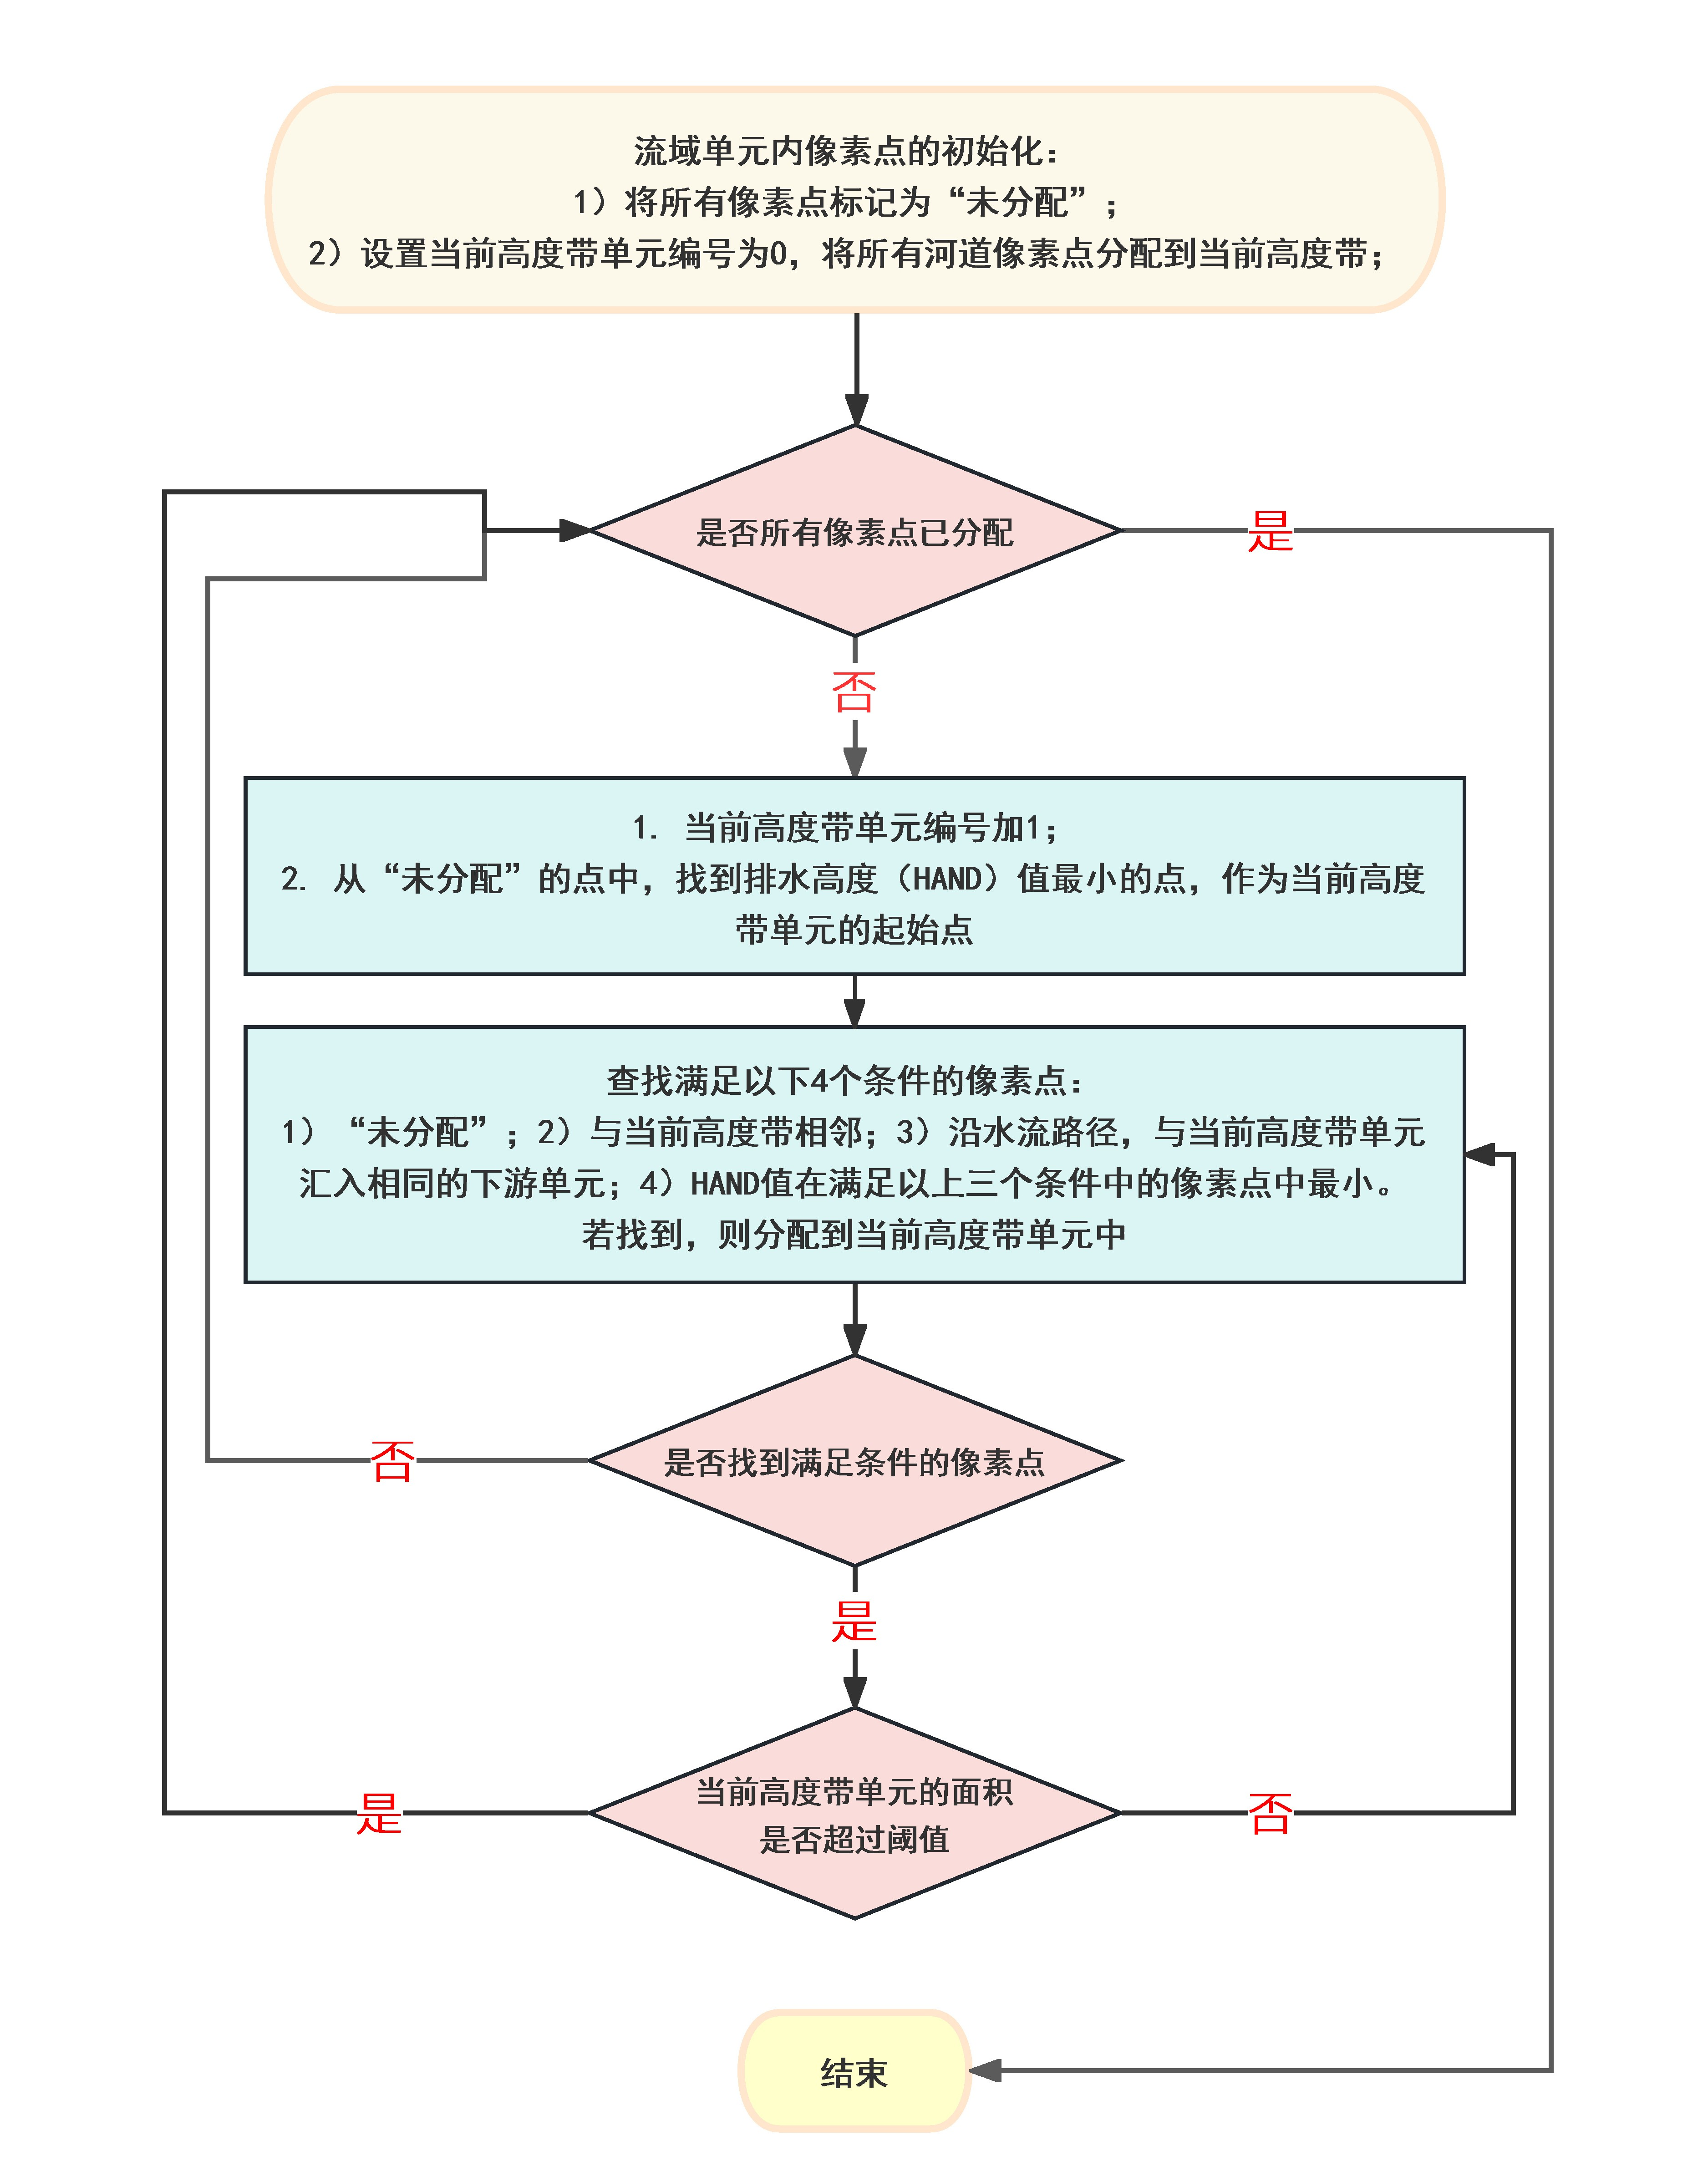
\includegraphics[width=0.8\textwidth]{Figures/模式构架/高度带单元划分算法.jpg}
    \caption{高度带单元划分算法流程图}
    \label{fig:高度带单元算法流程}
  \end{figure}
}

图~\ref{fig:高度带单元约束示意}~显示了对高度带单元的划分进行上述约束的作用。仅使用HAND数据进行高度带单元的划分时,会产生空间上不连通的单元(图~\ref{fig:高度带单元约束示意}b~中的6号和7号单元),一个高度带单元的不同部分在地理位置上可能相隔较远,增加连通性约束后,可避免这种情形。

{
  \begin{figure}[htbp]
    \centering
    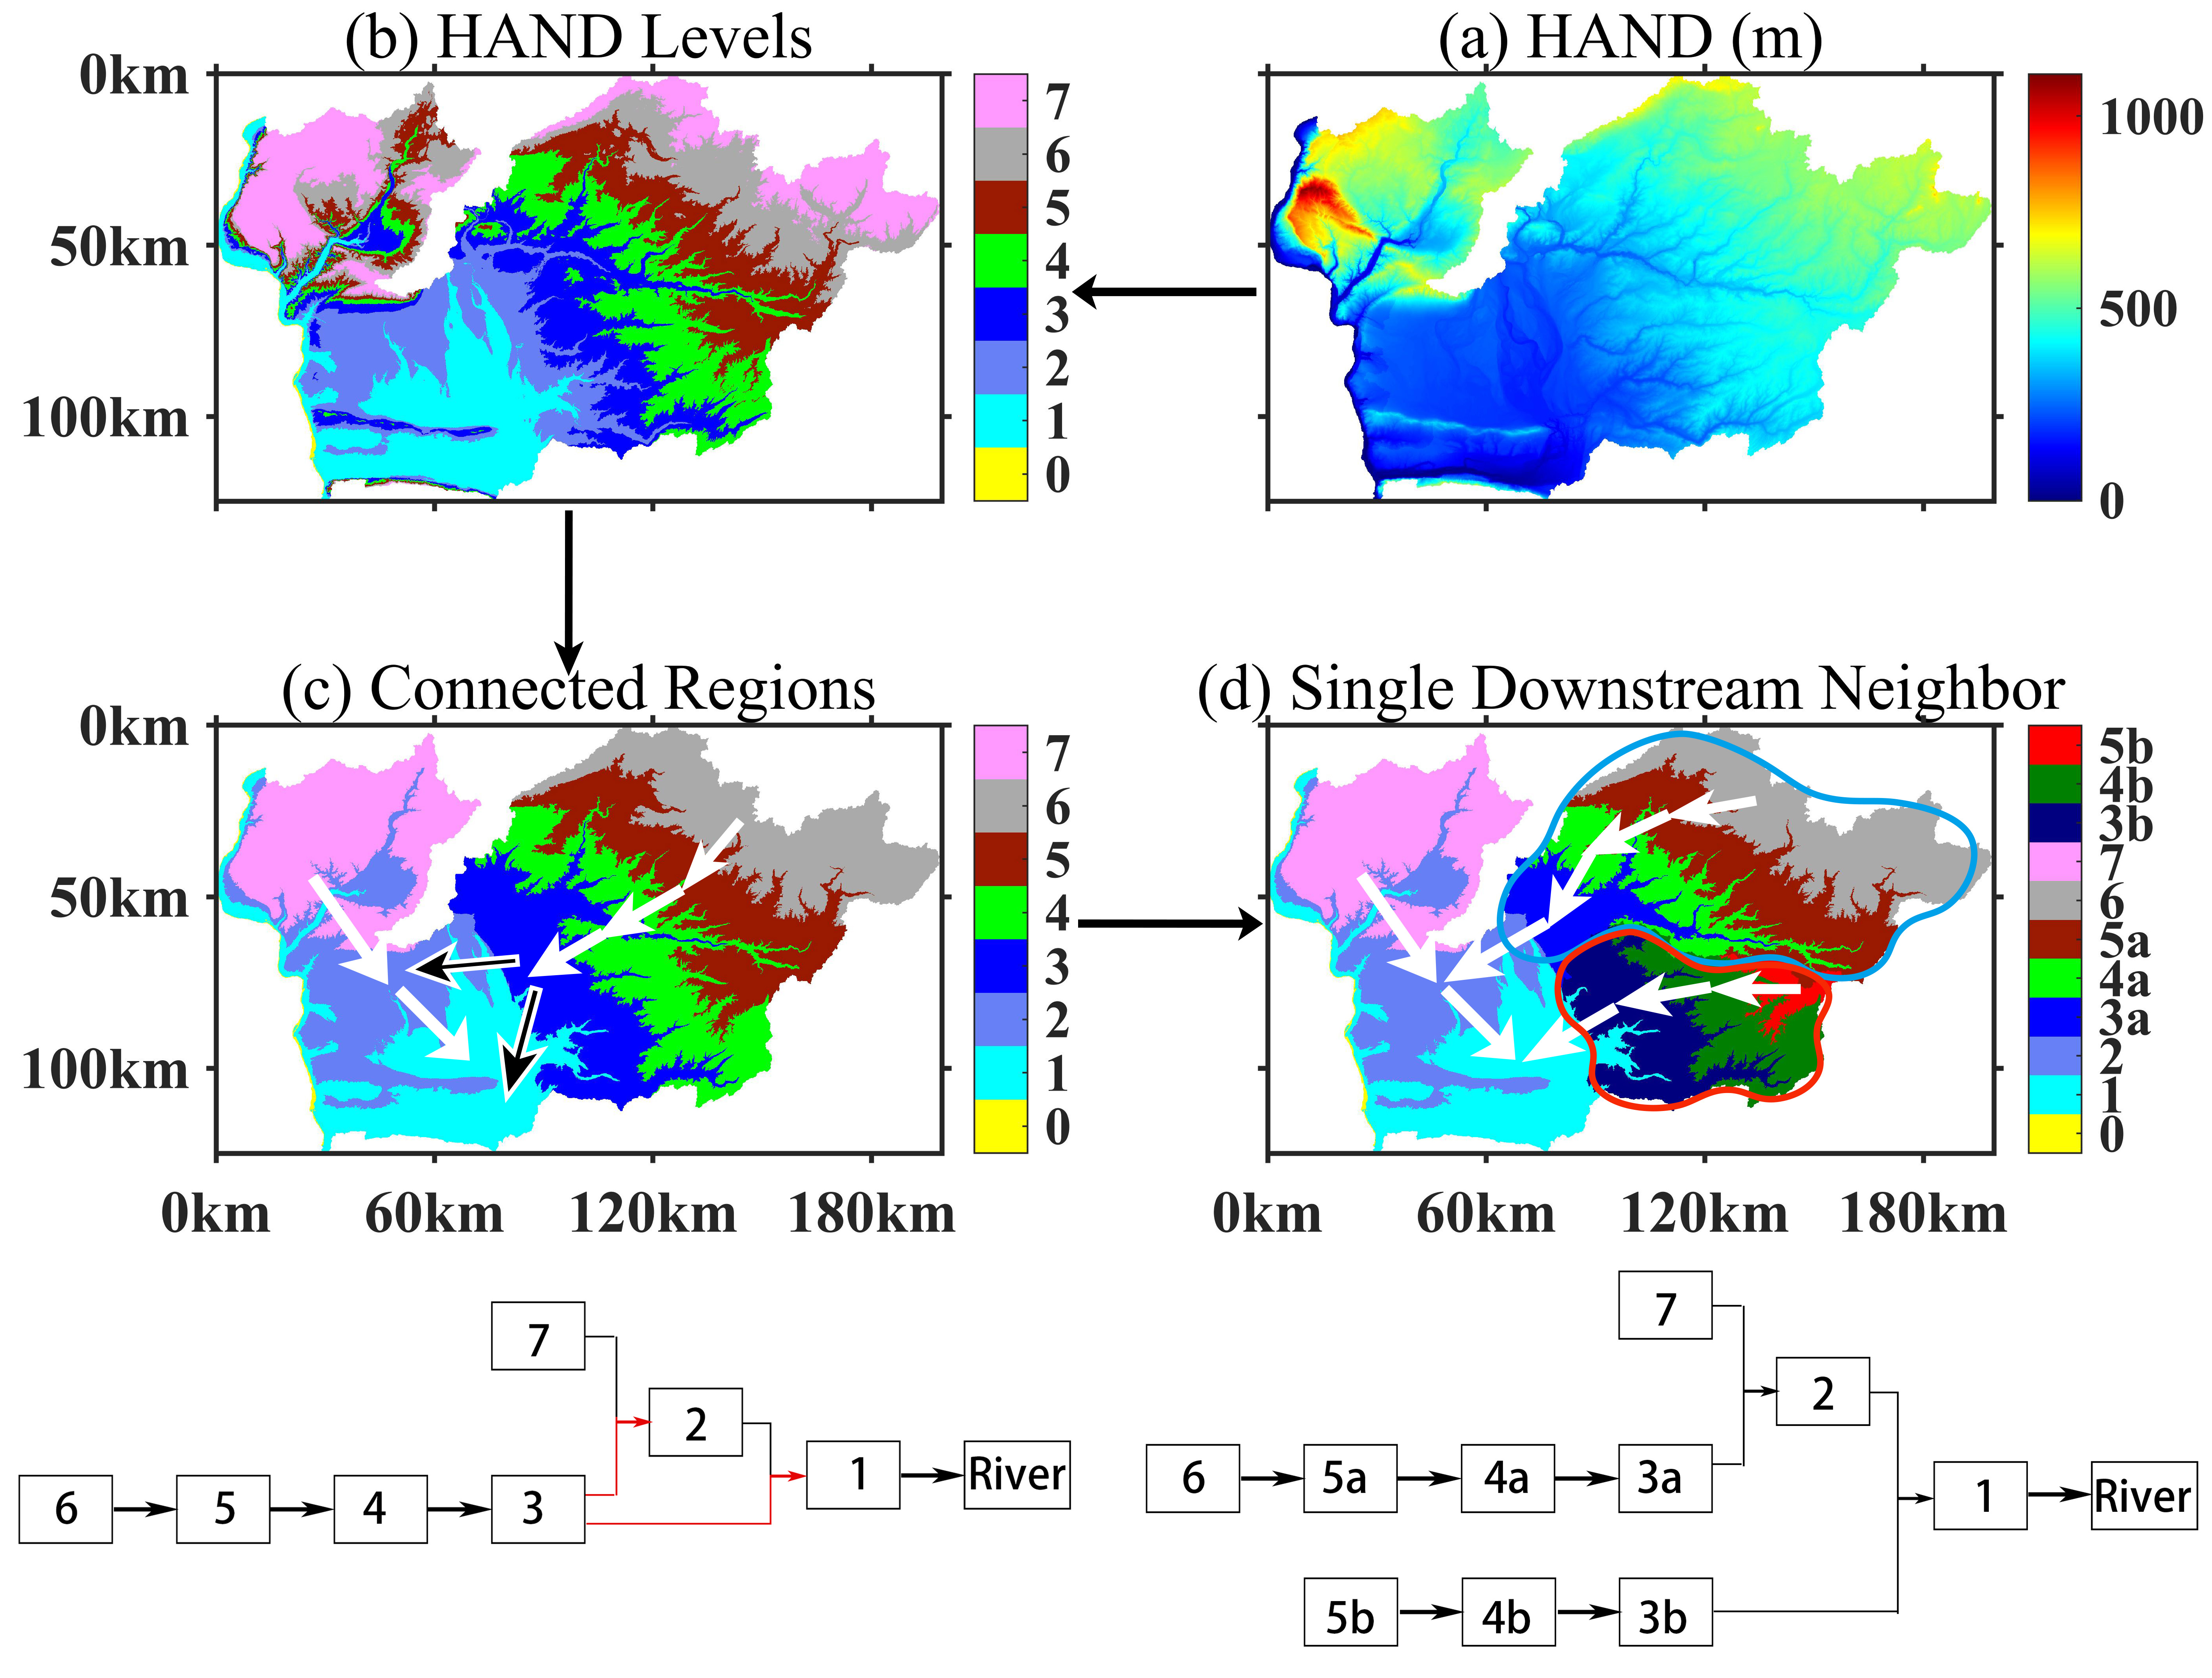
\includegraphics[width=\textwidth]{Figures/模式构架/高度带单元的约束示意图.jpg}
    \caption[对高度带单元进行约束的作用]{对高度带单元进行约束的作用:a)排水高度(HAND);b)仅根据排水高度划分高度带单元;c)具有连通性的高度带单元;d)满足连通性和具有唯一下游单元的高度带单元。上图中的箭头表示水流的方向}
    \label{fig:高度带单元约束示意}
  \end{figure}
}

在流域单元网格中,每个流域单元关联了一段河道。目前未考虑河道向下游分叉的情况,因此,除入海口和内陆洼地单元外,每个流域单元都有唯一的下游单元,整个模拟区域的流域单元在水文上都是连通的(见图~\ref{fig:湖泊划分}~左)。

自然连通的湖泊设置为独立的单元,不受面积阈值的限制。生成流域单元网格时,首先使用HydroLAKES数据\citep{messager2016nc}将区域内的湖泊标识出来,再将模拟区域内的其余部分划分为流域单元。为了避免单个湖泊的面积过大,使用CVT算法\citep{du1999siam}对湖泊进行了进一步的划分(见图~\ref{fig:湖泊划分}~右)。
{
  \begin{figure}[htbp]
    \centering
    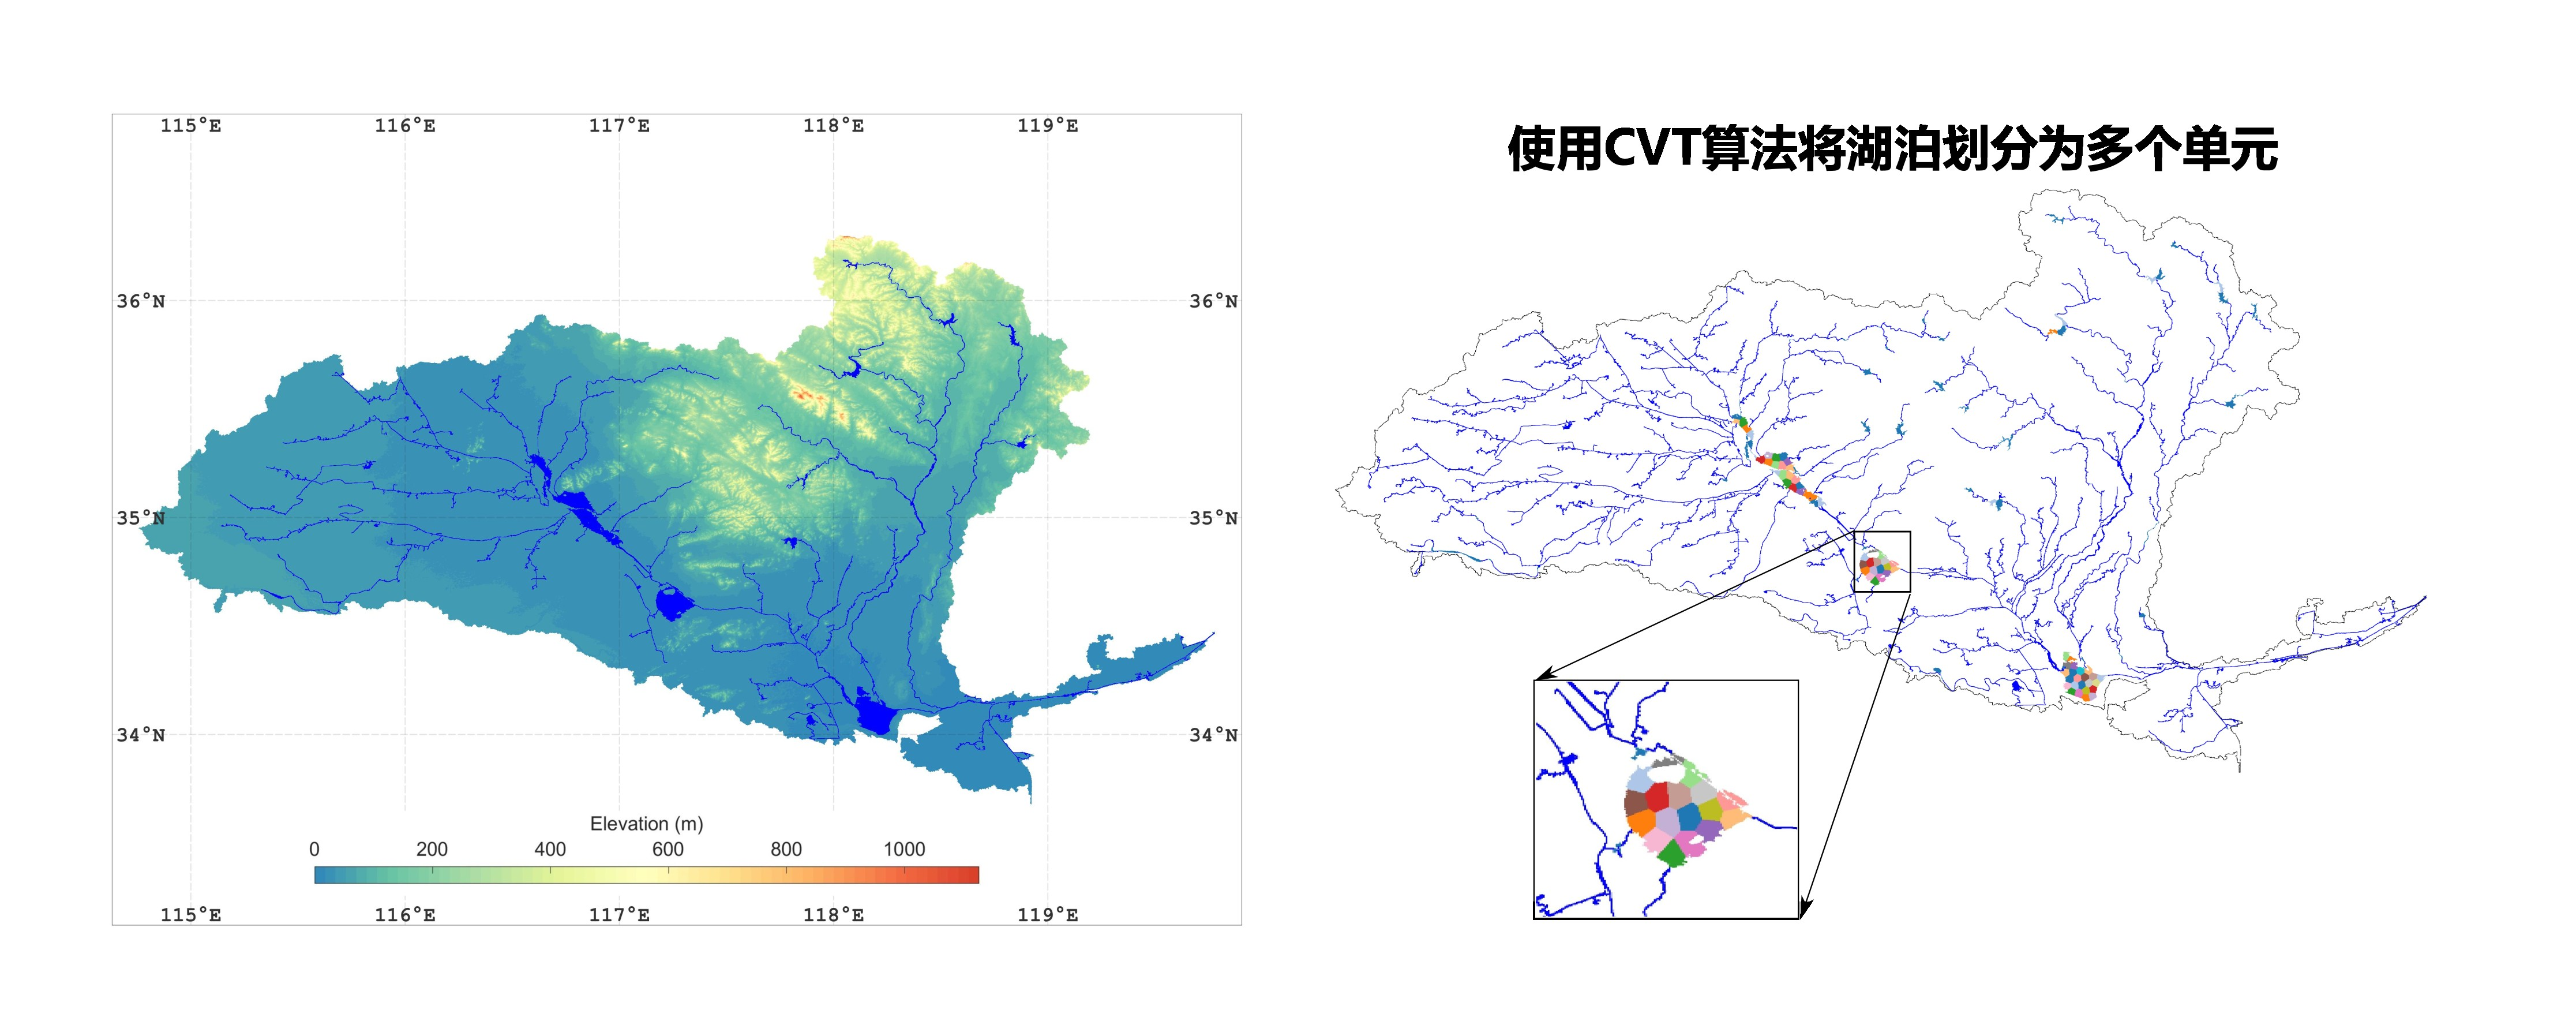
\includegraphics[width=\textwidth]{Figures/模式构架/湖泊划分.jpg}
    \caption[流域单元网格中的湖泊]{流域单元网格中的湖泊。左图为模拟区域(淮河流域)的范围、高程以及河道和湖泊网络。右图表示采用CVT算法将湖泊区域进一步划分为更小的单元}
    \label{fig:湖泊划分}
  \end{figure}
}



\section{次网格结构}\label{次网格}
\esection{Subgrid Structure}
\begin{mymdframed}{代码}
  本节对应的次网格类型可在\texttt{/include/define.h}中进行选择。
\end{mymdframed}
\subsection{次网格结构概述}
\esubsection{Overview of Subgrid Structure}
考虑到地表下垫面覆盖的异质性,CoLM对模式网格单元进一步划分次网格。
次网格是CoLM计算模拟的基本结构单元,通常称为patch(斑块)。
Patch是通过使用高分辨率的精细化网格数据,根据网格单元内部地表覆盖类型、植被功能类型、叶面积指数、土壤属性和地形等分布特征,按一定方式进行划分并聚合而来。Patch主要是用于模拟网格单元内部不同下垫面覆盖的过程(即对地表异质性的考虑),同时也起到了减少计算量的作用。


由patch可以组成按经纬度网格、流域单元网格(章节~\ref{流域单元网格})及非结构网格(章节~\ref{非结构网格})。
在patch尺度计算得到的通量按其所在网格覆盖比例进行面积加权平均,作为地表网格通量模拟结果。
地表状态或预报变量一般情况下亦是如此,在patch尺度计算得到的结果按照面积加权平均后作为模式结果输出。

{
  \begin{figure}[htbp]
    \centering
    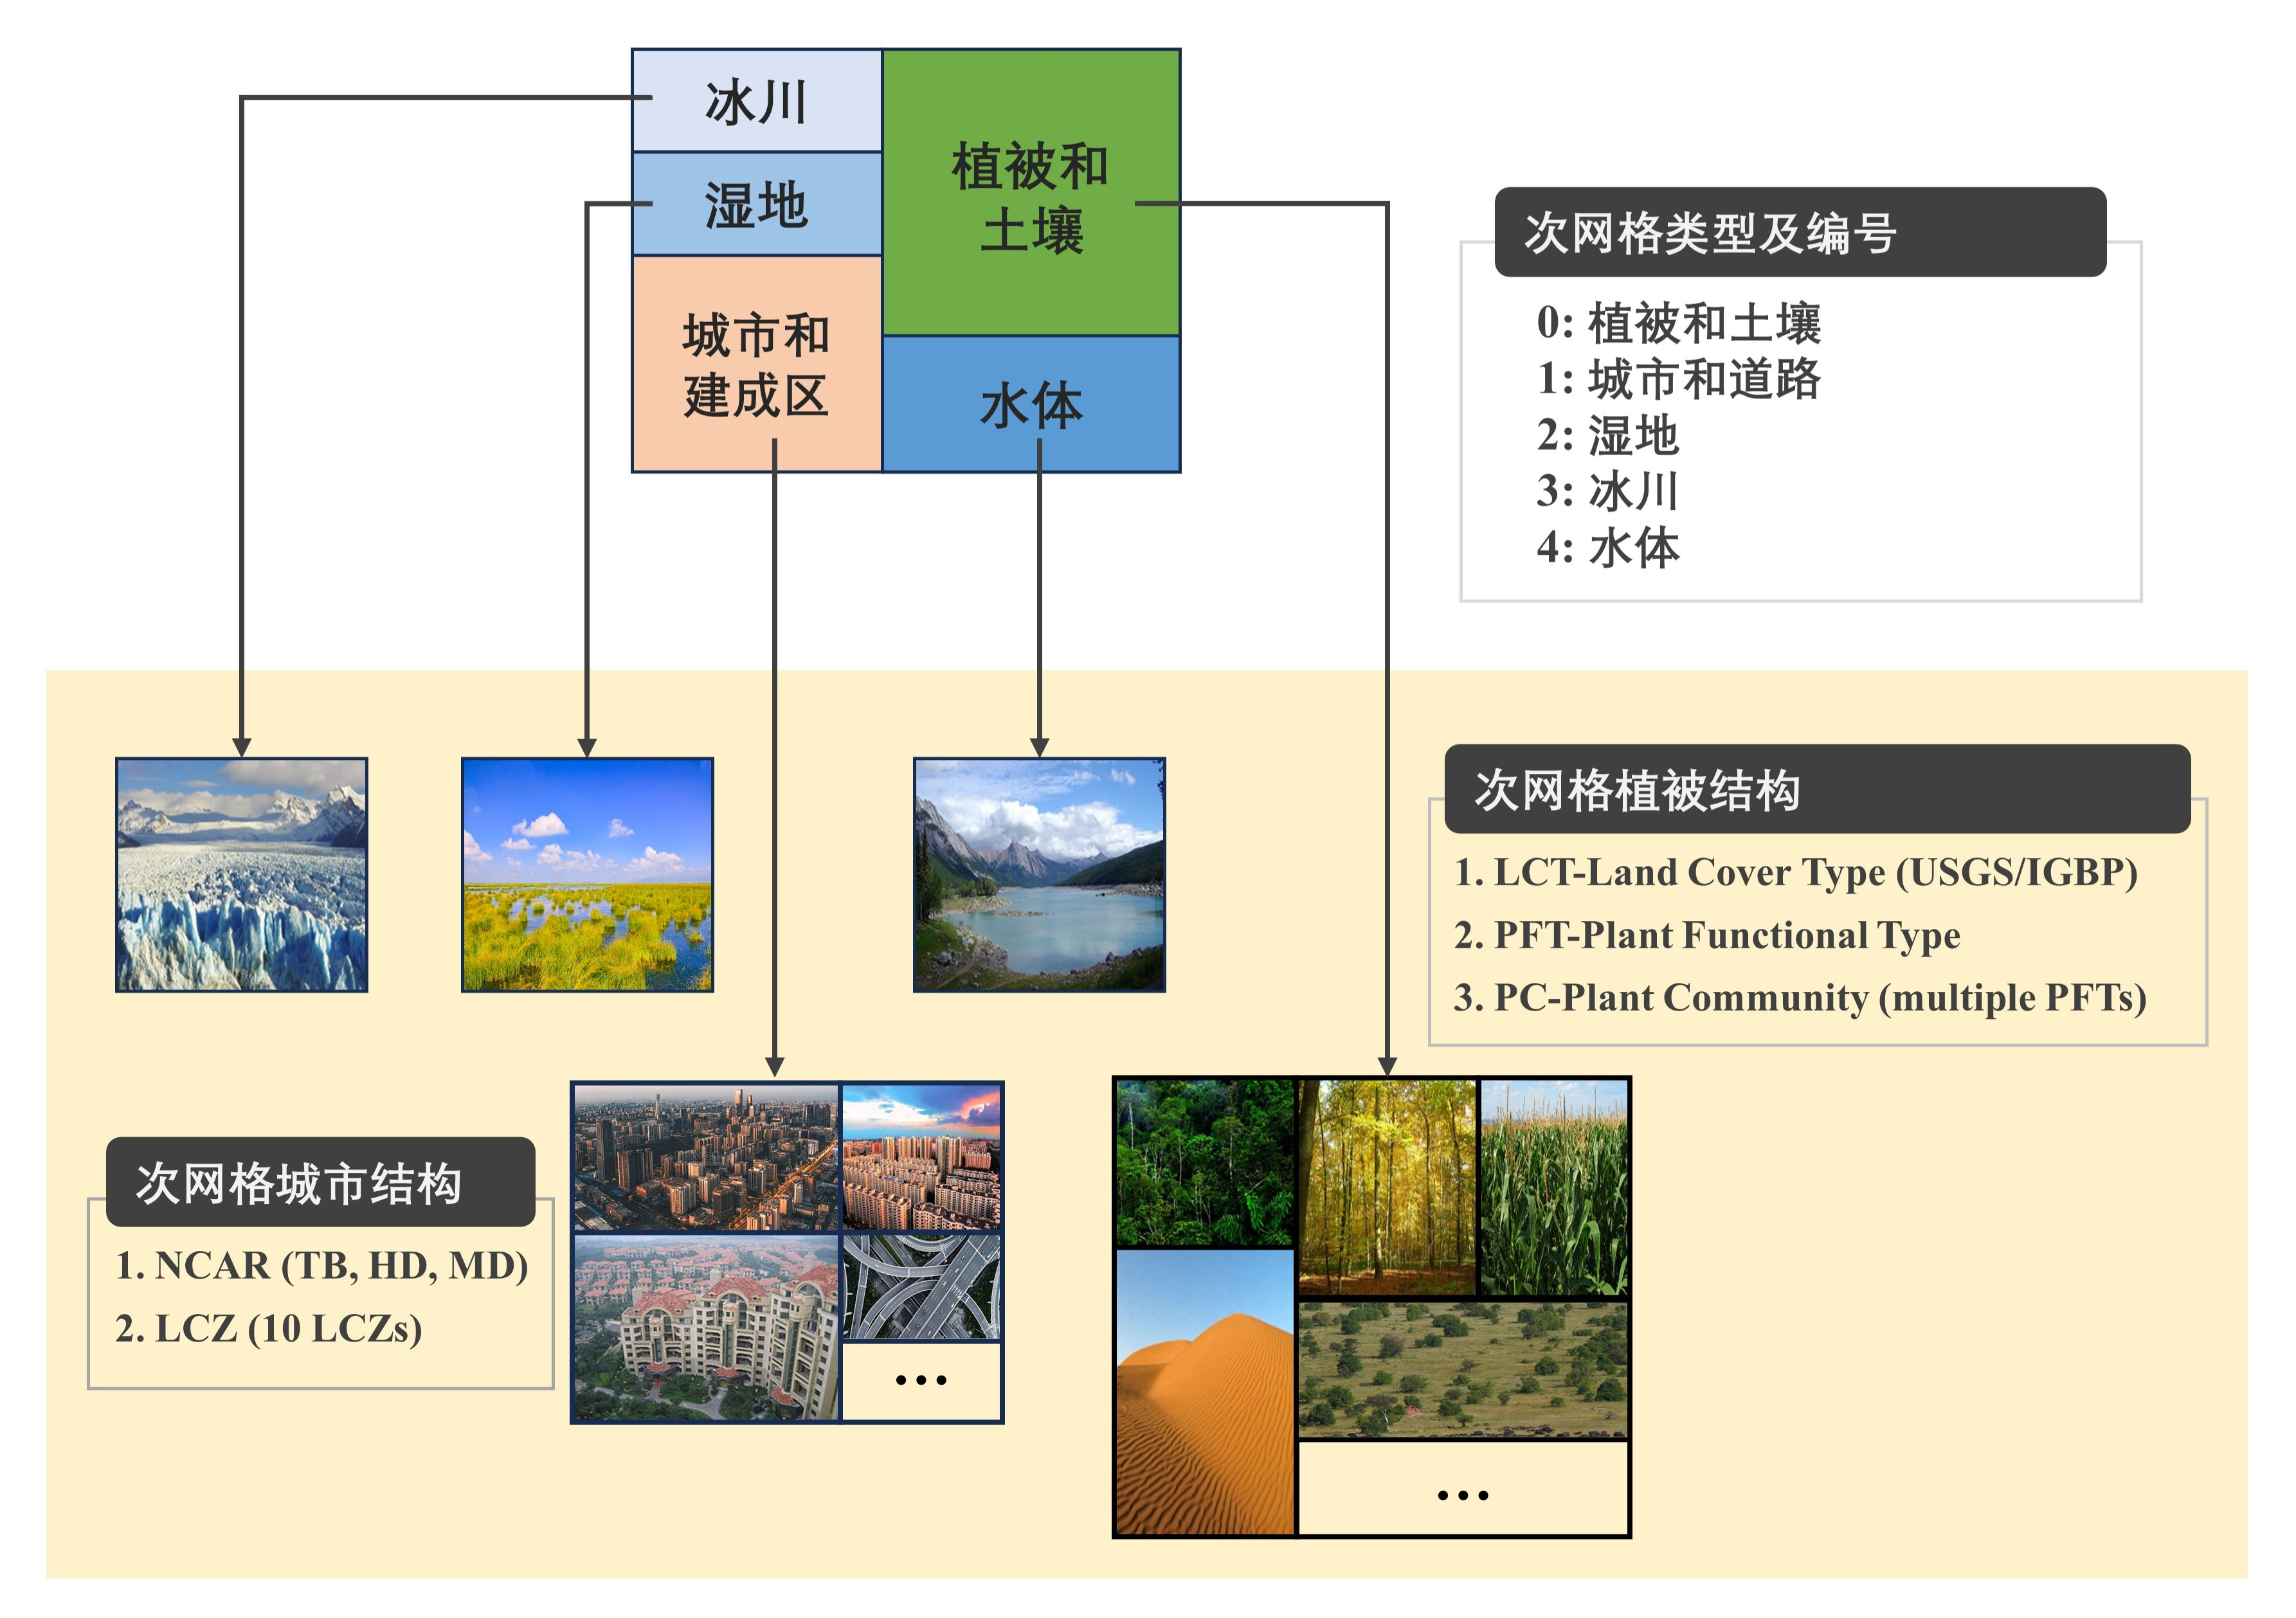
\includegraphics[width=\textwidth]{Figures/模式构架/CoLM次网格结构示意图_v4.jpg}
    \caption[CoLM次网格结构示意图]{CoLM次网格结构示意图。次网格植被(Sub-grid vegetation)结构提供三种可选方式:LCT, PFT以及PC;当作物模式打开时,每种作物当成一种独立的PFT (CFT)进行模拟;当城市模式打开时,次网格城市(Sub-grid urban)结构提供两种可选方式:NCAR 3种城市分类和LCZ 10种分类}
    \label{fig:次网格结构示意图}
  \end{figure}
}


CoLM非海洋patch从大类上分为五类:植被(含裸土)、城市、湿地、冰川和水体,如图~\ref{fig:次网格结构示意图} 所示。在模式中的编号依次为0--4。其中植被和城市patch可根据不同类型进一步细分。

\subsection{植被次网格结构}\label{sec:植被次网格}
\esubsection{Vegetation Subgrid}
植被patch可以分为自然植被和作物。自然植被patch采用三种可选次网格植被结构进行表征(图~\ref{fig:植被次网格方案}):1) 地表覆盖类型---LCT (Land Cover Type);2) 植被功能型---PFT (Plant Function Type)和3) 植物群落---PC (Plant Community)。以上三种方式,模式运行时只能选择其中一种。

{
  \begin{figure}[htbp]
    \centering
    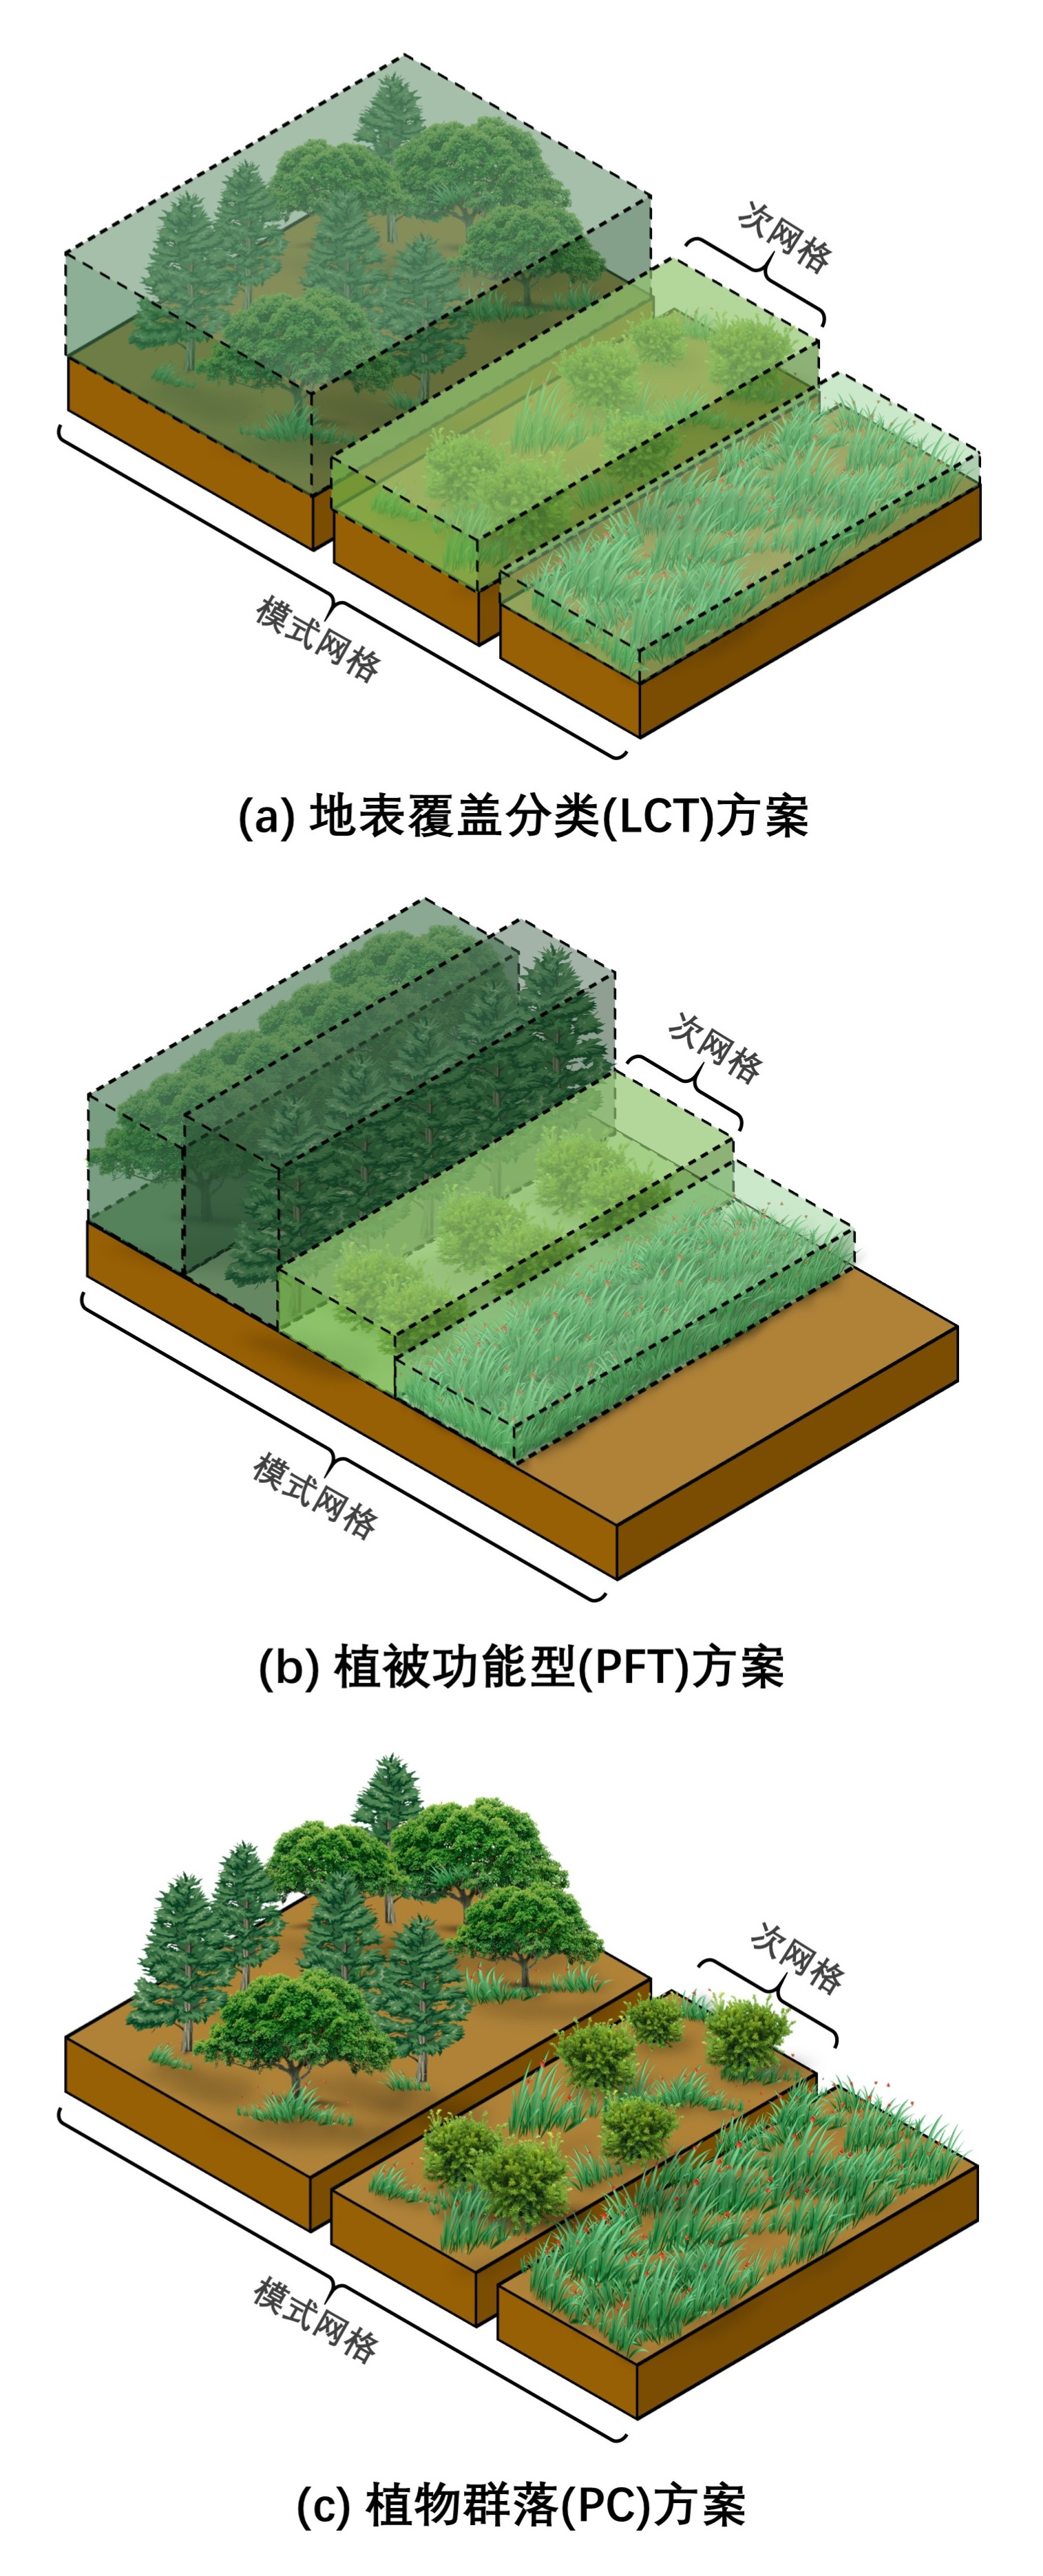
\includegraphics[width=0.55\textwidth]{Figures/模式构架/植被次网格方案示意图_v4.jpg}
    \caption[CoLM植被次网格方案示意图]{CoLM植被次网格方案示意图。图中a (LCT方案)、b (PFT方案)中虚线框蒙版表示其包含的植被结构水平均一;图c (PC方案)与图a的差别在于缺少虚线框所示蒙版,即对次网格中的植被结构进行显式表达}
    \label{fig:植被次网格方案}
  \end{figure}
}

1. LCT次网格方案

LCT方案为CoLM2014版原有方案(图~\ref{fig:植被次网格方案}a所示),即将某一地表覆盖类型可能包含的多种功能型植被当成混合(水平均一)植被进行模拟,其设置的相关参数可视为等效参数。图~\ref{fig:植被次网格方案}a中虚线框所示蒙版表示其中所包含植被结构水平均一。例如热带大草原地表覆盖类型,虽然可能同时包含树和草,但仍视为一种植被,因此相应的植被参数只有一套。

2. PFT次网格方案

PFT是目前陆面模式(如CLM和JULES)常采用的次网格表征方式,也是本版本CoLM新添加的方式(图~\ref{fig:植被次网格方案}b所示)。
PFT方案是将每一个细网格地表覆盖类型进行拆解,得到其PFT的组成种类和各自面积占比,并将其聚合到模式网格中。同样,每种PFT植被结构也假设为水平均一,在图~\ref{fig:植被次网格方案}b中用虚线蒙版表示。本版本CoLM默认PFT方案类似于CLM PFT方案,即模式格点中的所有PFT作为1个植被patch,共享土壤水热等环境,但各PFT的辐射和通量等过程计算相对独立。同时,CoLM也提供每种PFT完全独立的方案,即土壤水热等环境模拟也保持独立。

{
  \begin{figure}[htbp]
    \centering
    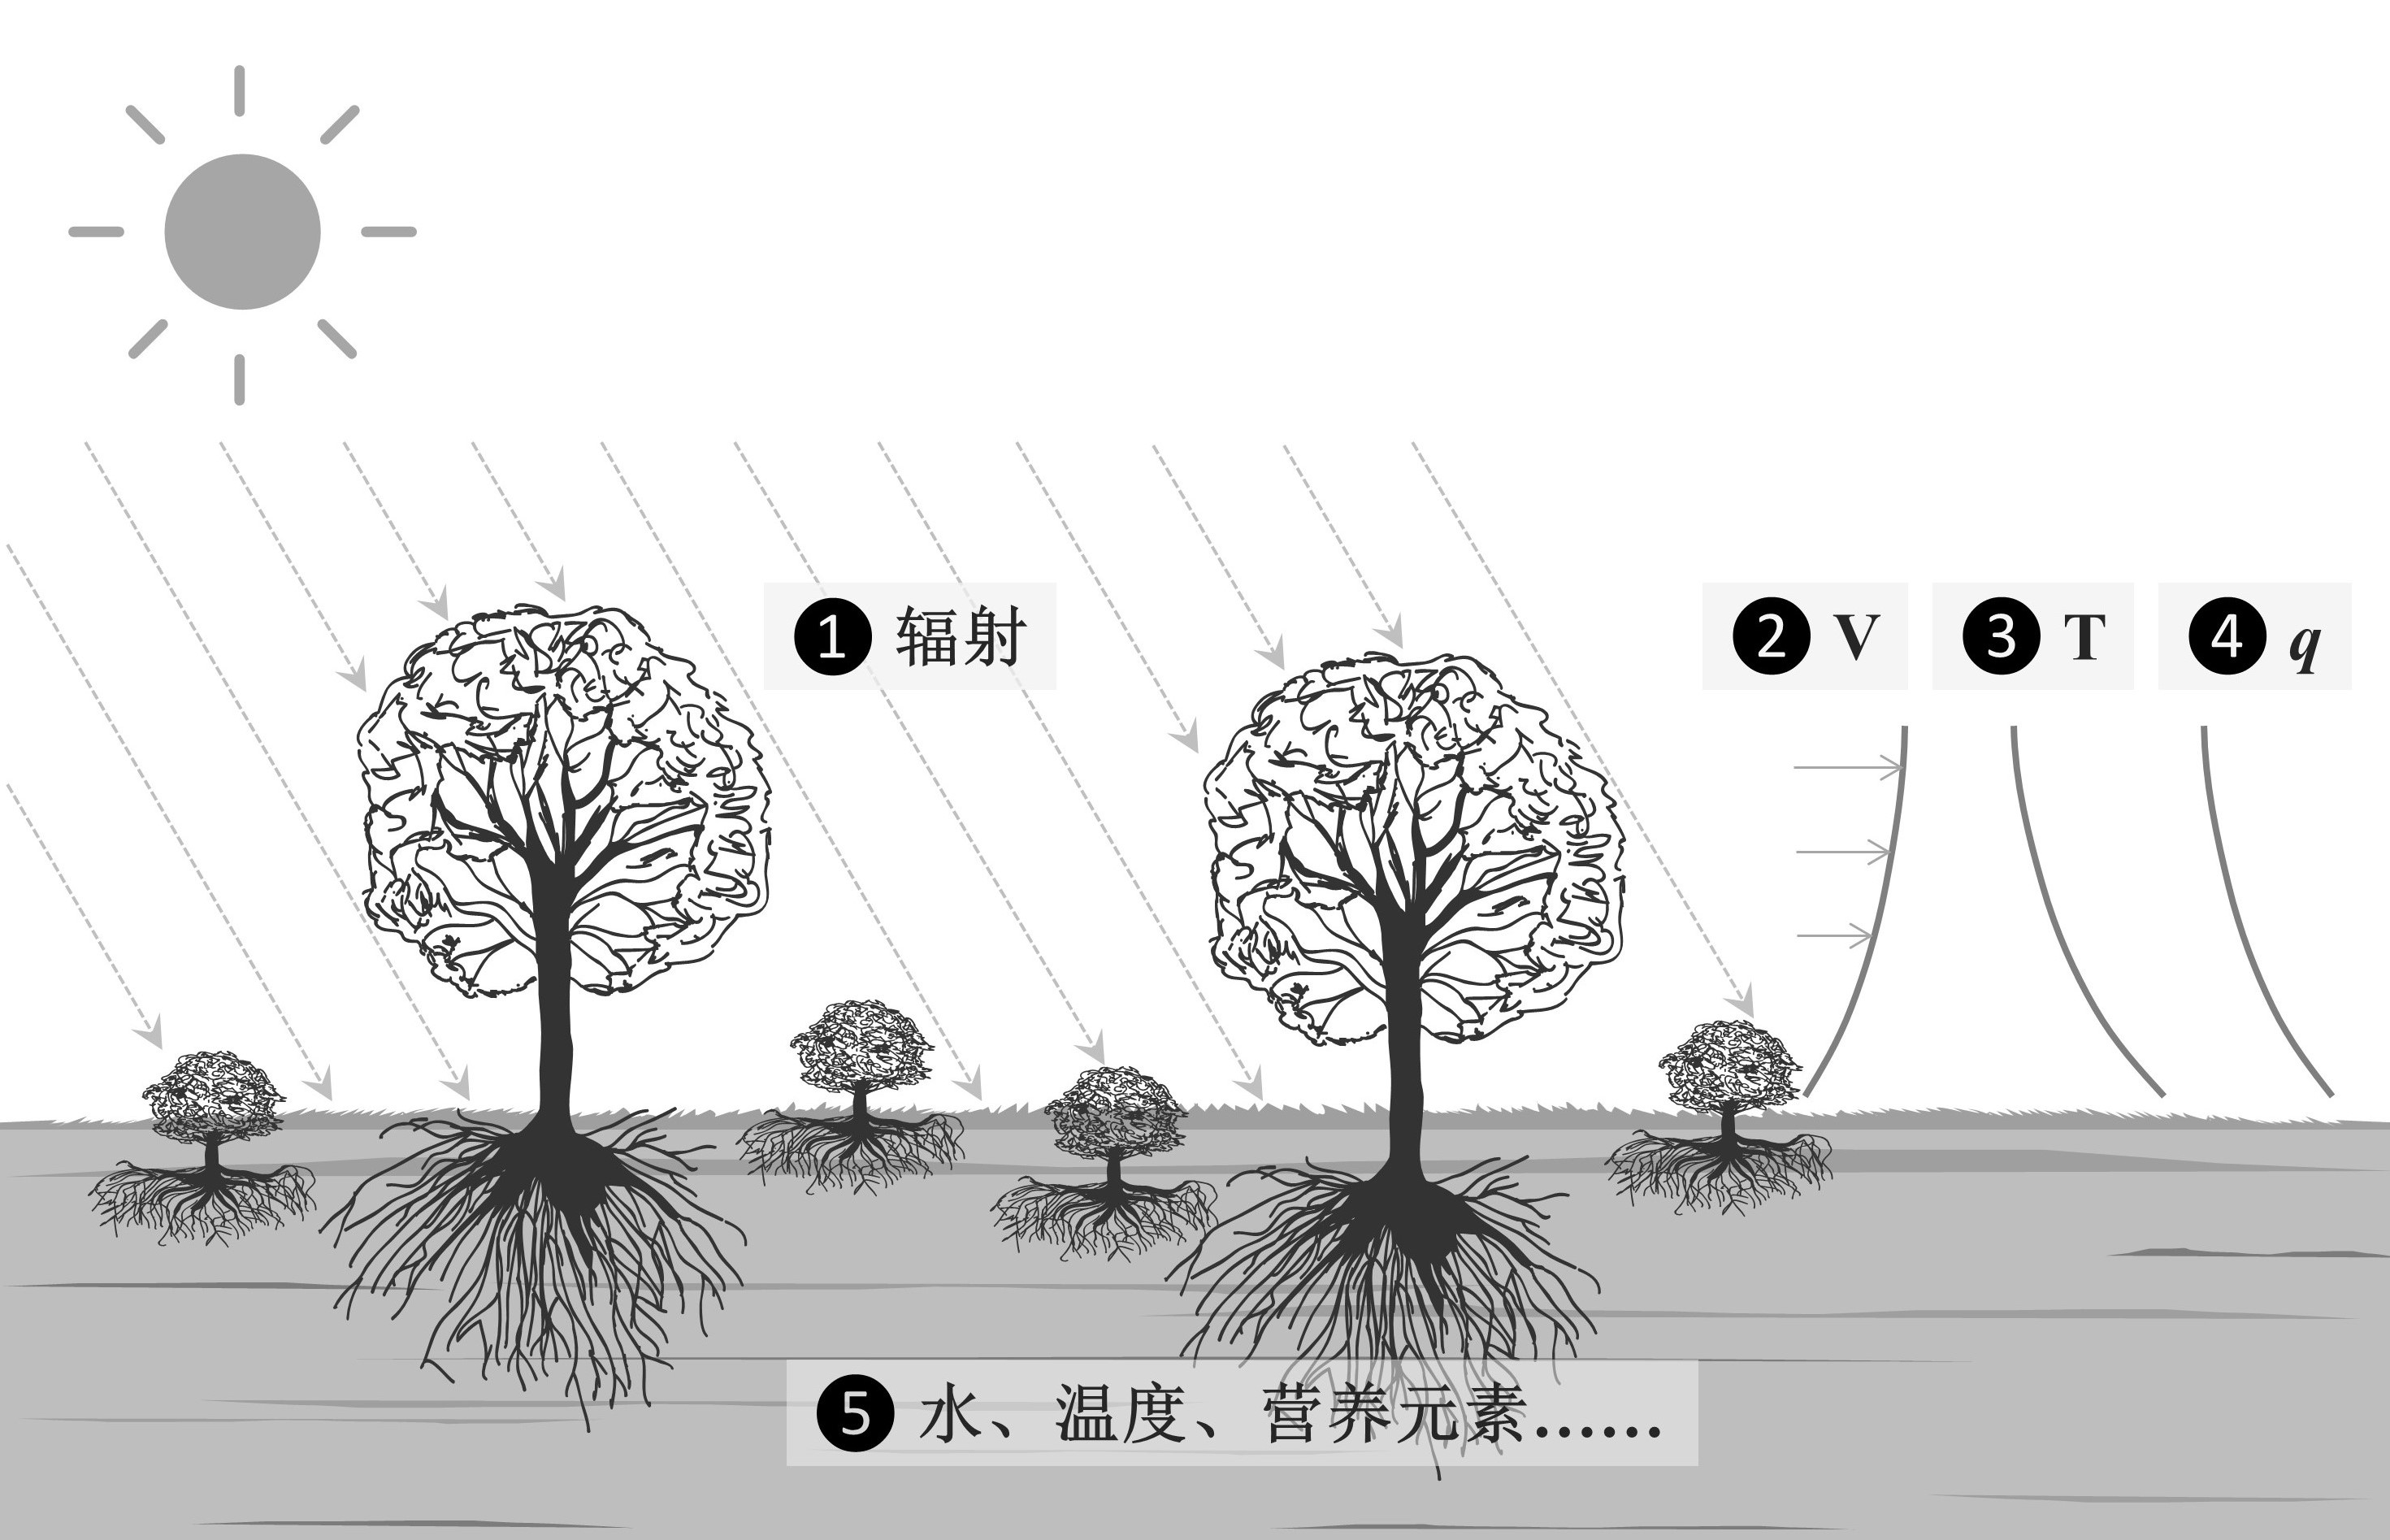
\includegraphics[width=0.95\textwidth]{Figures/模式构架/植物群落示意图_v2.jpg}
    \caption[CoLM植物群落(PC)次网格概念示意图]{CoLM植物群落(PC)次网格概念示意图。同一植物群落中的PFT环境共享,资源竞争,包括辐射、风速、水热及营养元素等}
    \label{fig:植物群落示意图}
  \end{figure}
}

3. PC次网格方案

PC方案保留LCT方案中模拟对象,即地表覆盖类型,同时还进一步对LCT中的地表覆盖植被类型进行PFT细分(图~\ref{fig:植被次网格方案}c所示)。
不同于LCT方案把某一类型地表覆盖的所有植被视为混合植被,PC方案对某一地表覆盖类型所组成的每种PFT进行显式表达计算,所有PFT在同一次网格patch中共享辐射、风、水热及营养元素等环境,即辐射和通量计算等过程中PFT之间相互影响、同时求解,显式地考虑了PFT之间的共存与竞争(如图~\ref{fig:植物群落示意图} 所示)。这一方案类似于植物群落的概念,故命名为PC (Plant Community)方案。

LCT方案所依赖的地表覆盖类型数据可以直接由USGS (章节~\ref{USGS地表覆盖数据})或者MODIS-IGBP地表覆盖数据获取(章节~\ref{IGBP地表覆盖数据})。PFT和PC方案所需要的植被结构及属性数据由MODIS-IGBP地表覆盖数据加以其他辅助数据制作而成。

对于作物patch,当作物模式未打开时,作物被当成一种特殊的自然植被进行模拟;当打开作物模式时,每个模式格点根据包含的作物分类及组成比例(外部数据读取)分别建立相互独立的patch进行模拟计算,方式类似PFT方案,但不同之处在于每种作物的土壤计算保持独立,不共享土壤水热等环境。

\subsection{城市次网格结构}
\esubsection{Urban Subgrid}
\begin{mymdframed}{代码}
  本节对应的城市次网格类型可在\texttt{MOD\_Namelist.F90}中进行选择。
\end{mymdframed}

城市patch与作物类似,当城市模式未打开时,城市被当成一种地表覆盖进行模拟,即薄板城市模型(Slab Urban);
当城市模式打开时,每个模式格点根据包含的城市类型和组成比例分别建立相互独立的patch进行模拟计算。

{
  \begin{figure}[htbp]
    \centering
    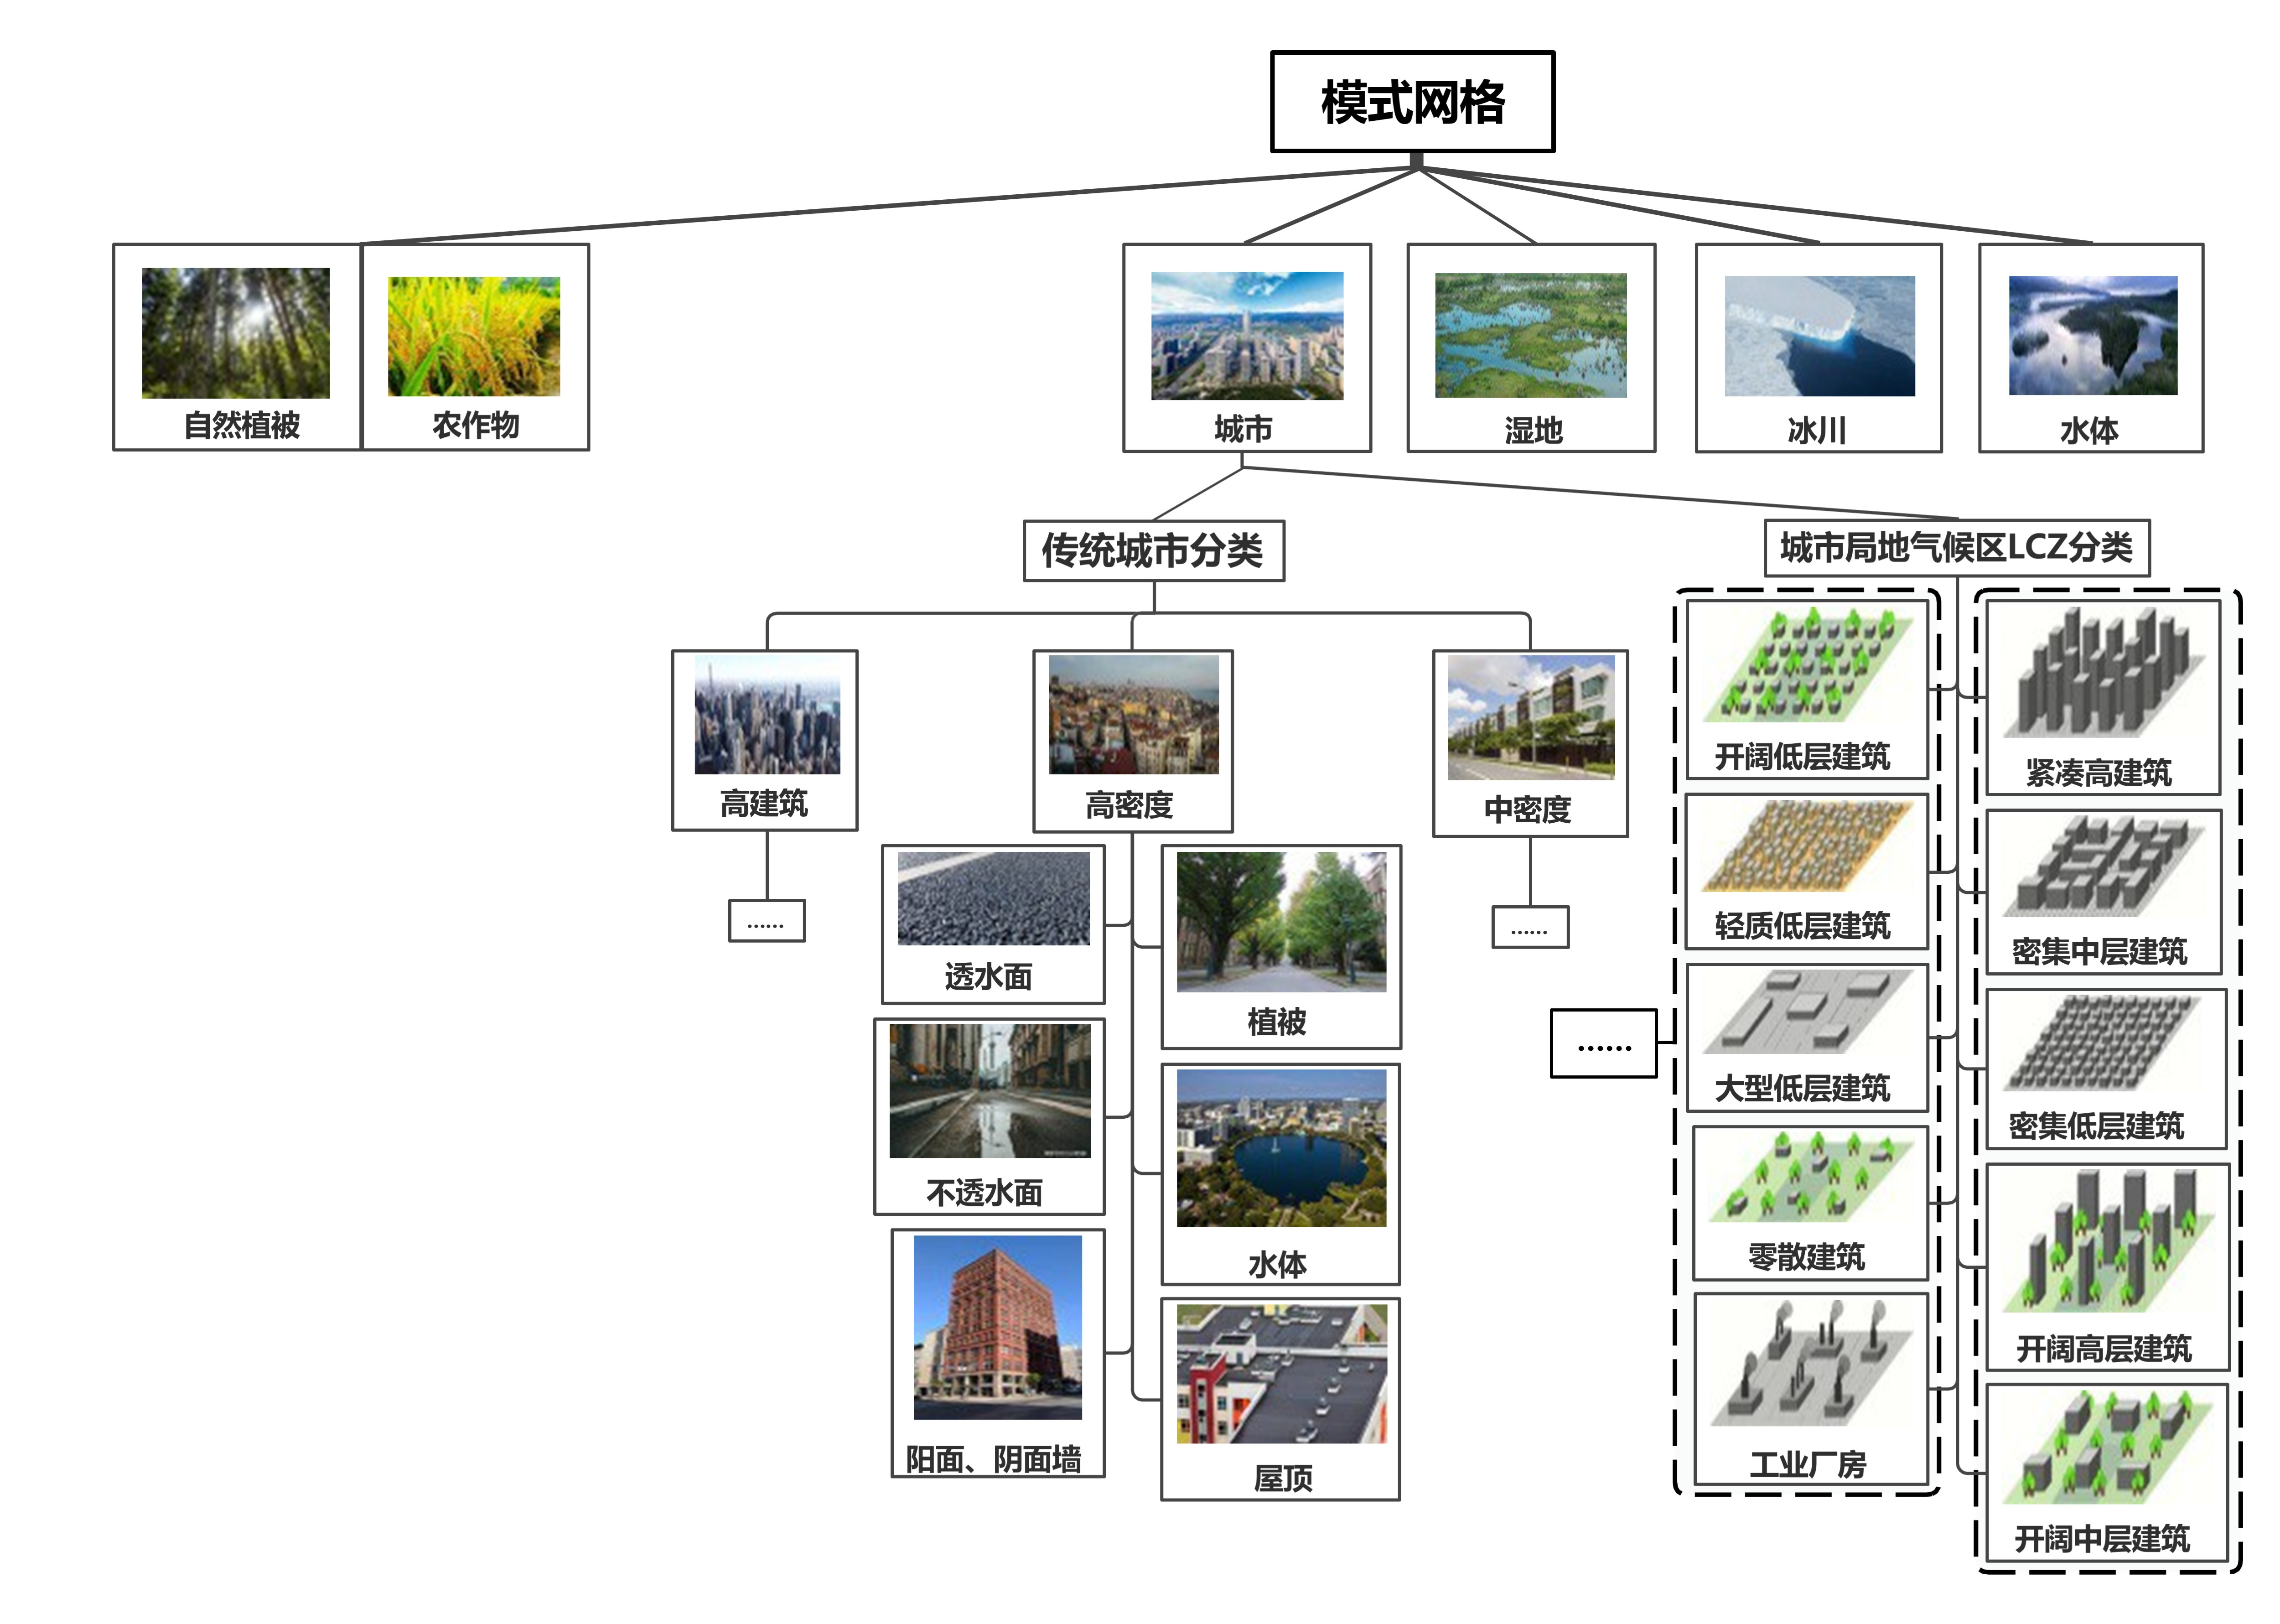
\includegraphics[width=0.95\textwidth]{Figures/模式构架/CoLM城市次网格示意图.jpg}
    \caption[CoLM城市模式次网格结构示意图]{CoLM城市模式次网格结构示意图}
    \label{fig:城市次网格}
  \end{figure}
}

目前城市分类提供两种方式(图~\ref{fig:城市次网格}):
\begin{enumerate}
  \item 根据城市密度分为高建筑-TB、高密度-HD和中密度-MD 3类(基于NCAR CLMU城市模式);
  \item 根据城市局地气候区(LCZ,Local Climate Zone)分为10类。
\end{enumerate}
每种城市类型由屋顶、不透水地面、透水地面、阴/阳面墙、植被和水体组成。不透水地面和透水地面在后面章节中分别简称为不透水面和透水面。
城市分类及其相关属性数据主要从外部文件读取(章节~\ref{城市数据})。

\section{植被、土壤和积雪的垂直分层}\label{土壤和积雪的垂直分层}
\esection{Vertical Stratification}

{
  \begin{figure}[htbp]
    \centering
    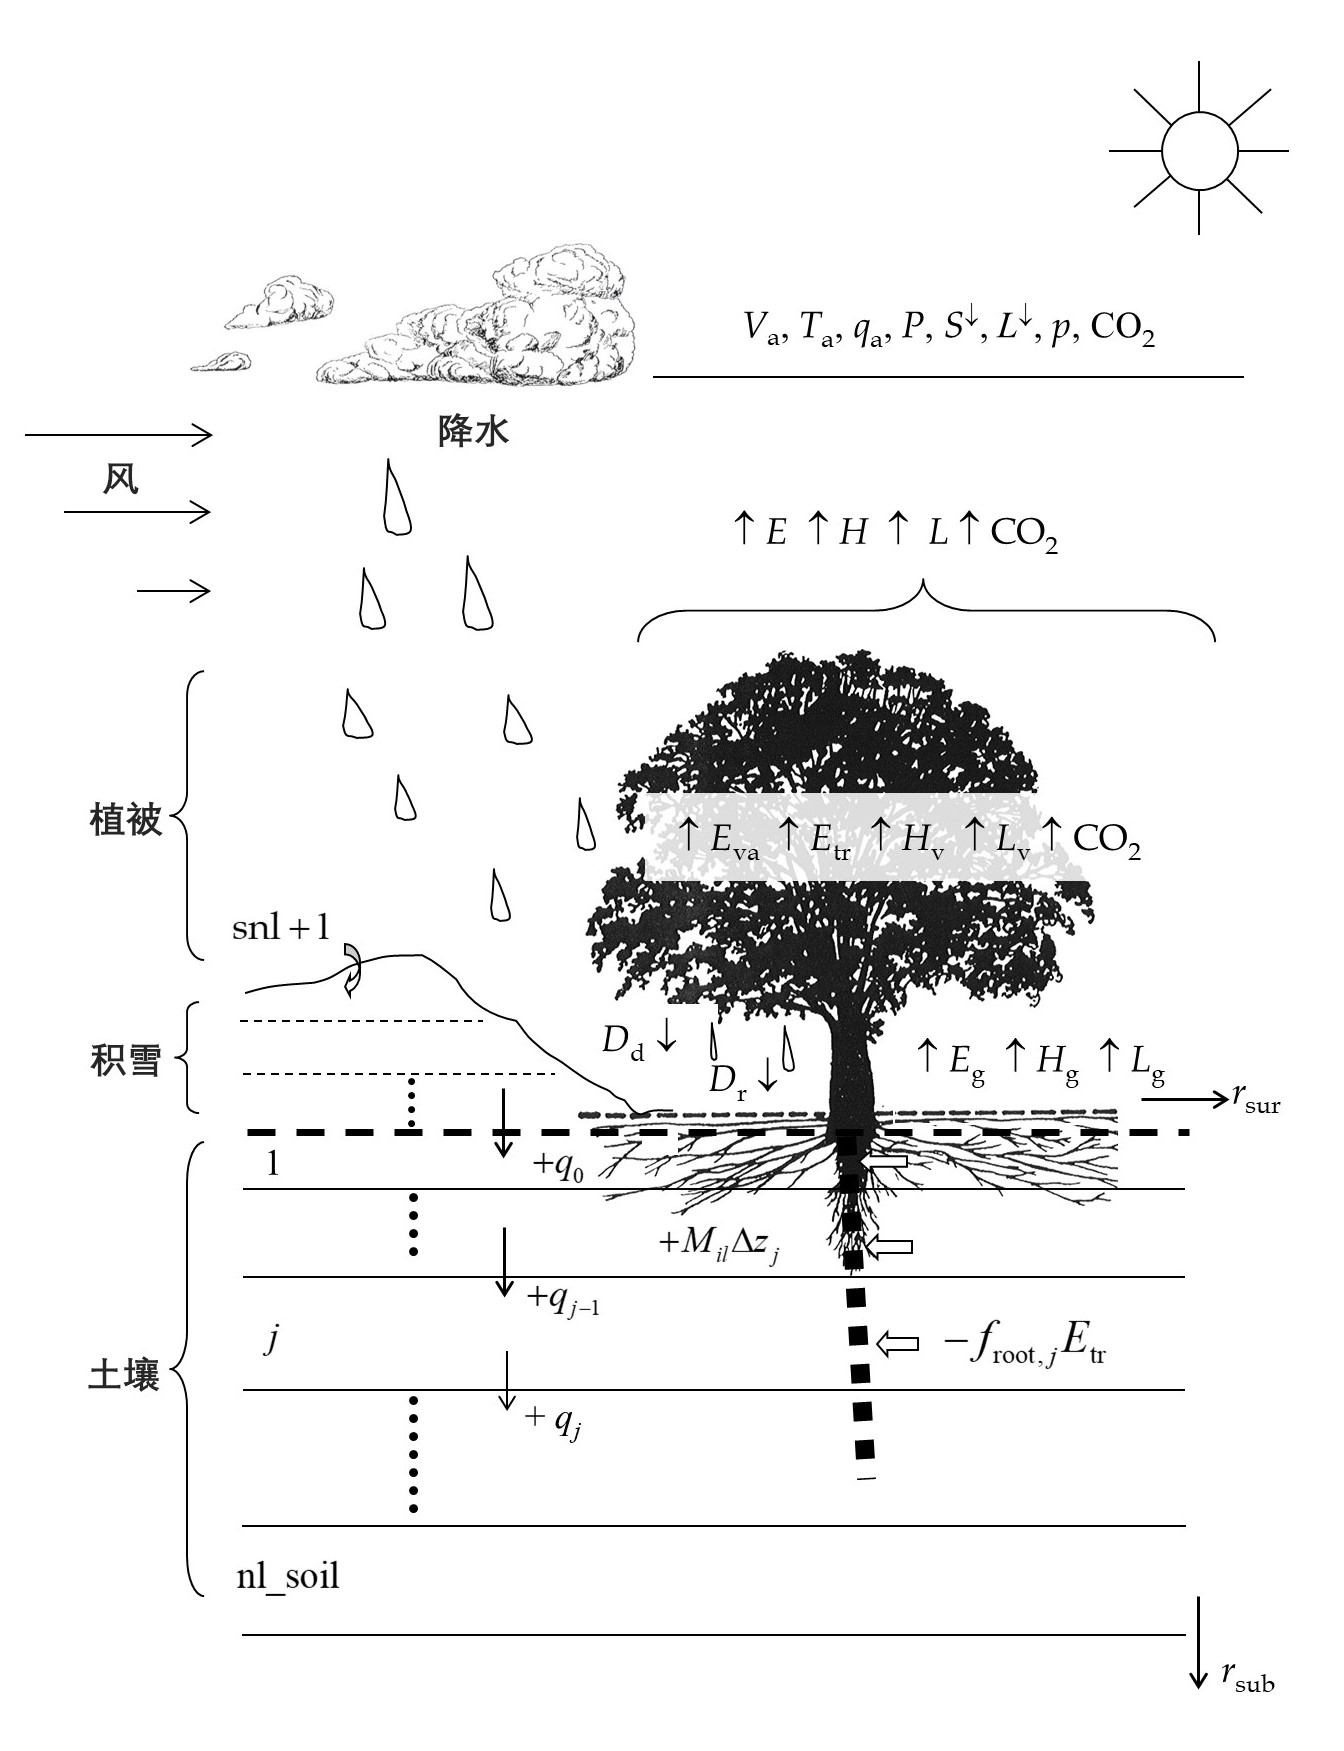
\includegraphics[width=0.9\textwidth]{Figures/模式构架/CoLM模式概念图_v2.jpg}
    \caption[CoLM植被、土壤和积雪垂直分层示意图]{CoLM植被、土壤和积雪垂直分层示意图}
    \label{fig:CoLM垂直分层}
  \end{figure}
}

CoLM植被、土壤和积雪的垂直分层如图~\ref{fig:CoLM垂直分层} 所示。

CoLM可根据次网格类型(章节~\ref{sec:植被次网格})将植被按照单层或最多三层进行模拟。对于单层植被(LCT和PFT植被次网格),采用双大叶模型进行模拟\citep{dai2004two};对于多层植被(PC植被次网格),每层植被的各PFT采用三维植被模型(章节~\ref{三维植被辐射传输模型} 和~\ref{三维植被湍流}),并结合双大叶模型进行模拟。

CoLM默认将土壤分为10层,每一层土壤的节点深度$z_i$~(m)定义为:
\begin{equation}\label{eq:z_soi}
  z_{i} = f_{\mathrm{s}}\left\{ \exp{\left\lbrack 0.5(i - 0.5) \right\rbrack} - 1 \right\}
\end{equation}
其中尺度因子$f_{\mathrm {s}}=0.025$. 因为土壤水热梯度在接近土壤与大气的交界面时往往较大,采用指数定义可以保证土壤接近表面时得到更细的分层。每一层土壤的厚度$\Delta z_i$~(m)计算为:
\begin{equation}
  \Delta z_{i}=\left\{\begin{array}{ll}0.5\left(z_{1}+z_{2}\right) & i=1 \\
      0.5\left(z_{i+1}-z_{i-1}\right) & i=2, \ldots, 9 \\
  z_{10}-z_{9} & i=10\end{array}\right.
\end{equation}
相邻两层土壤交界处的深度$z_{\mathrm{h},i}$ (m)可计算为:
\begin{equation}
  z_{\mathrm{h},i}=\left\{\begin{array}{ll}0.5\left(z_{i}+z_{i+1}\right) & i=1, \ldots, 9 \\
  z_{10}+0.5 \Delta z_{10} & i=10\end{array}\right.
\end{equation}
CoLM中每层土壤中心的深度及每层下边界的深度见表~\ref{table:土壤分层}。

\begin{table}[b]
  \caption{CoLM中的土壤分层(单位:米)} \label{table:土壤分层}
  \centering \renewcommand{\arraystretch}{1.2} \footnotesize
  \begin{tabular}{ccccccccccc}
    \toprule
    层         & 1      & 2      & 3      & 4      & 5      & 6      & 7      & 8      & 9      & 10     \\
    \midrule
    中心位置   & 0.0071 & 0.0279 & 0.0623 & 0.1189 & 0.2122 & 0.3661 & 0.6198 & 1.0380 & 1.7276 & 2.8646 \\
    下边界位置 & 0.0175 & 0.0451 & 0.0906 & 0.1655 & 0.2891 & 0.4929 & 0.8289 & 1.3828 & 2.2961 & 3.4331 \\
    \bottomrule
  \end{tabular}
\end{table}


雪盖位于土壤之上,可根据其厚度划分为至多5层。为与土壤层编号一致,
这里与土壤表层相邻的雪层记为第0层,逐渐向上依次记为第 -1 层直至至多为第 -4 层。
记$snl$为划分的雪层总层数的相反数,则最上层雪层即为第$snl+1$层。记雪层的厚度为$z_{\mathrm{sno}}$,当$z_{\mathrm{sno}}<0.01$~(m)时,这时积雪较少,不单独划分为层,$snl=0$,当$z_{\mathrm{sno}}\geqslant 0.01$~(m)时,积雪分层的方案见图~\ref{fig:积雪分层}。

{
  \begin{figure}[htbp]
    \centering
    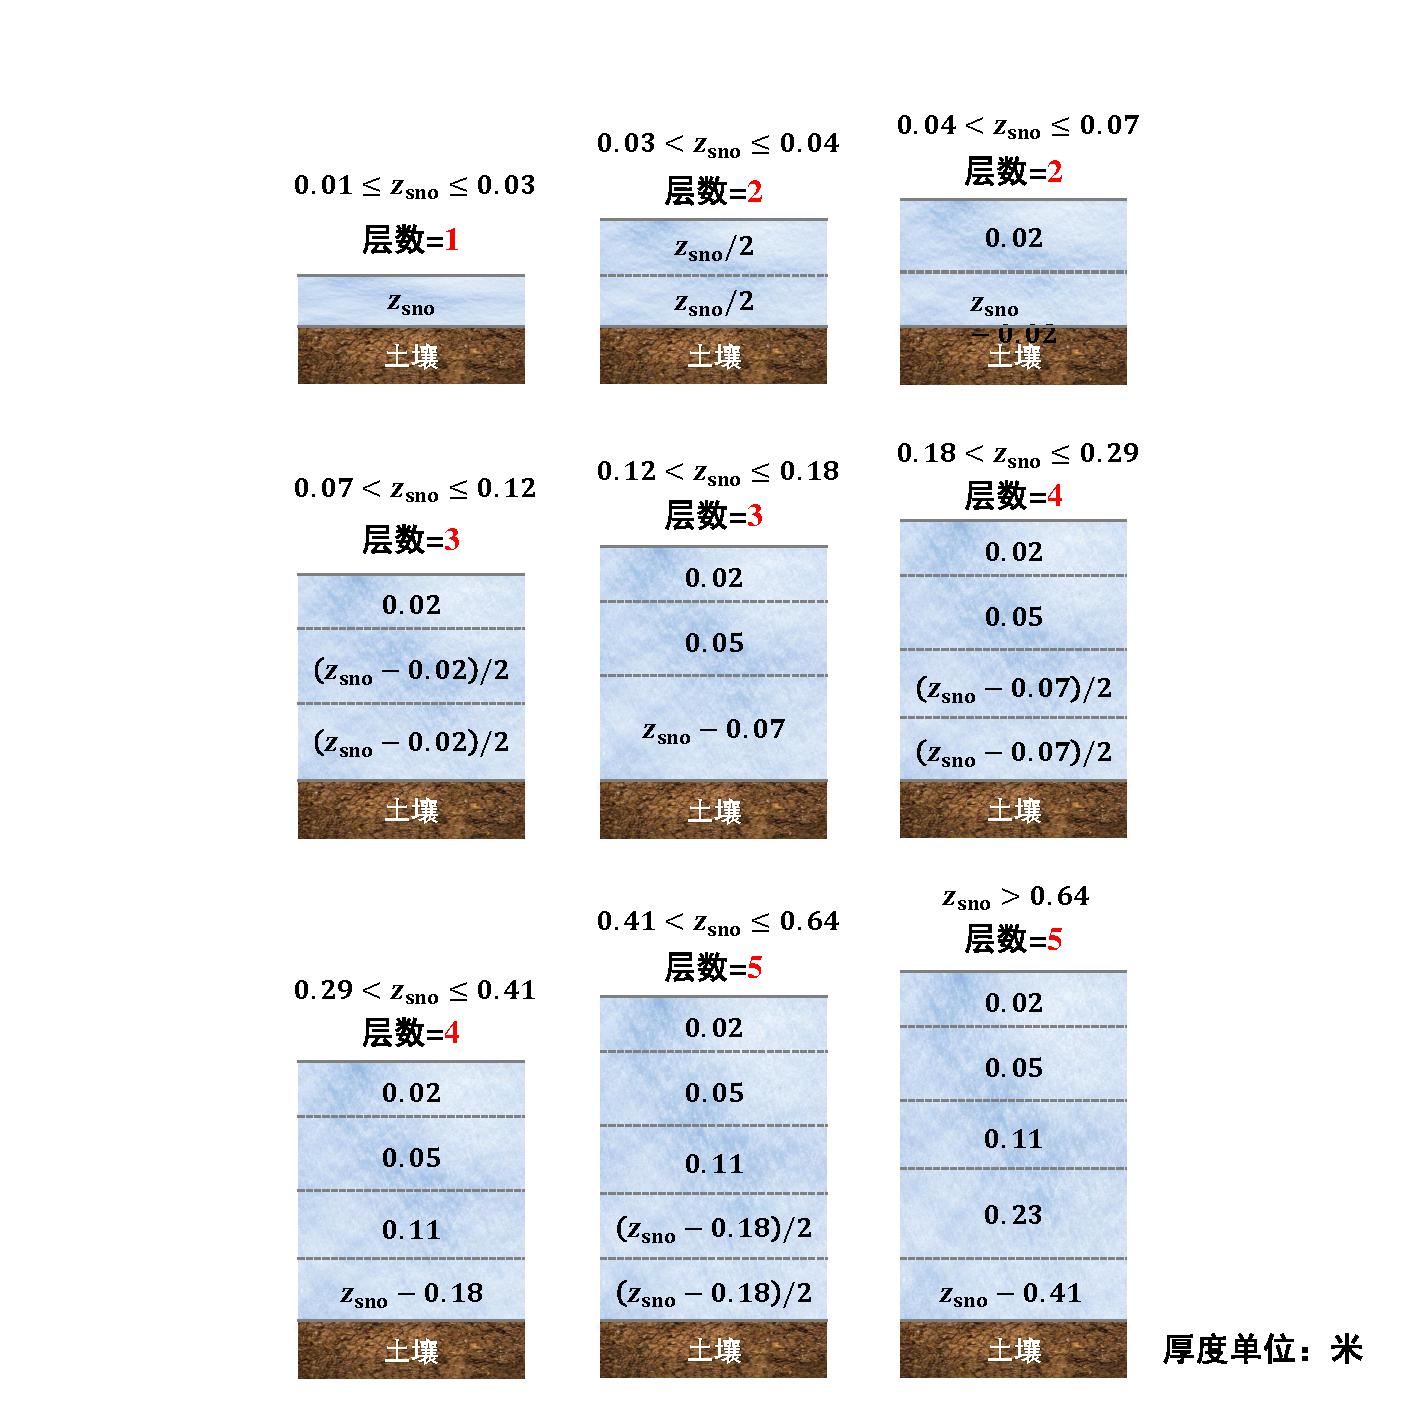
\includegraphics[width=0.95\textwidth]{CoLM-Latex/Figures/模式构架/积雪分层.pdf}
    \caption[CoLM积雪分层方案]{CoLM积雪分层方案。当$z_{\mathrm{sno}}<0.01 \unit{m}$时不形成积雪层,图中厚度单位为~\unit{m}}
    \label{fig:积雪分层}
  \end{figure}
}

$z_{\mathrm{h,0}}=0$为雪盖底层与土壤表层交界处的高度,$\Delta z_{i}$为第$i$层积雪的厚度。将交界面以上的高度定义为负值,则每一层雪的中心高度$z_i$~(m)与相邻两层雪交界处的高度$z_{\mathrm{h},i}$~(m)计算为:
\begin{equation}
  \begin{aligned}
    z_{i} &= z_{\mathrm{h},i}-0.5 \Delta z_{i} \quad i=0, \ldots, snl+1 \\
    z_{\mathrm{h},i} &= z_{\mathrm{h}, i+1}-\Delta z_{i+1}  \quad i=-1, \ldots, snl
  \end{aligned}
\end{equation}


\section{计算框架}\label{计算框架}
\esection{Computational Framework}

{
  \begin{figure}[htbp]
    \centering
    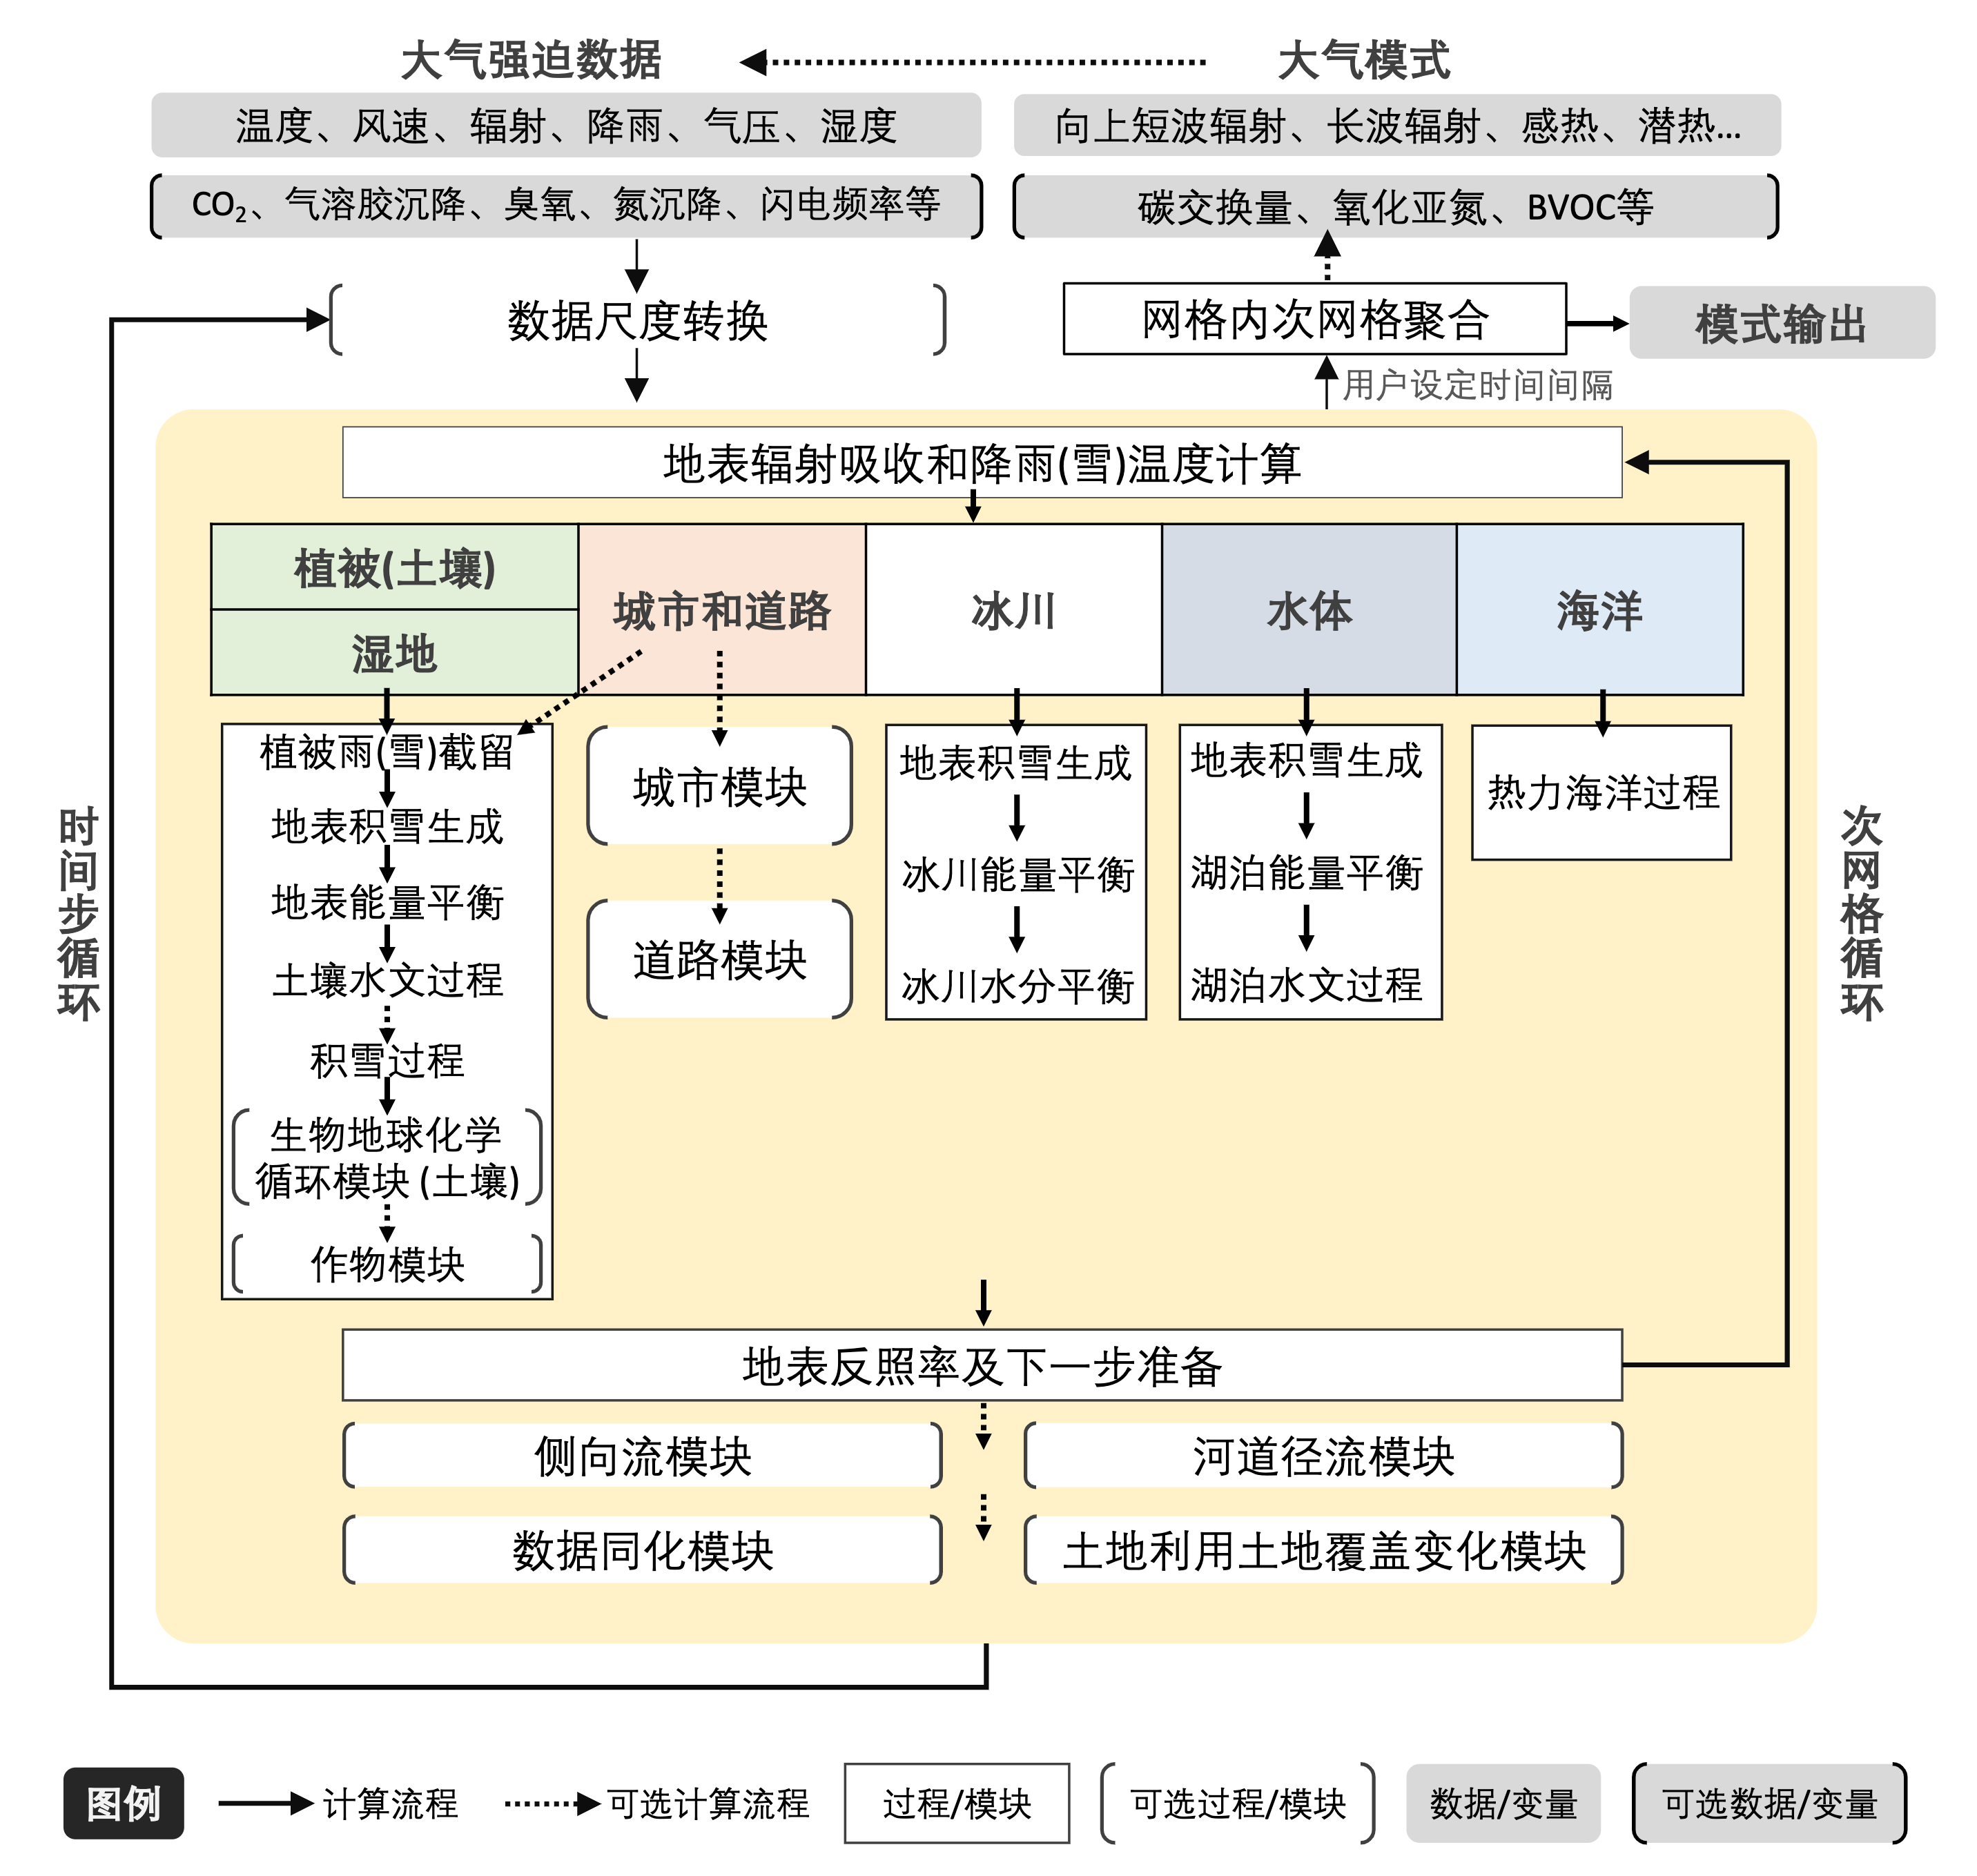
\includegraphics[width=\textwidth]{Figures/模式构架/CoLM计算框图_v7.png}
    \caption{CoLM计算框图}
    \label{fig:CoLM计算框图}
  \end{figure}
}

CoLM主程序计算流程主要包括模式数据的读取、时间步循环、次网格循环,以及模式数据输出(图~\ref{fig:CoLM计算框图})。涉及的过程主要在\texttt{main}文件夹下\texttt{CoLM.F90},\texttt{CoLMDRIVER.F90}及 \allowbreak \texttt{CoLMMAIN.F90}
\allowbreak (\texttt{URBAN\allowbreak /Urban\allowbreak \_CoLMMAIN.F90},当城市模式打开时)文件中进行调用。

\textbf{模式数据读取}大概可分为驱动数据和地表数据。其中驱动数据可以通过在离线模式下读取大气强迫数据,包括温度、风速、辐射、降雨等必要变量,以及气溶胶、氮沉降等可选变量,具体可参见表~\ref{tab:陆面模式所需的大气状态变量}。在读取过程中可根据需要进行适当数据尺度转换;如时间尺度不匹配,可进行简单时间维插值。另外,驱动数据也可以通过与大气模式耦合来获得。

\textbf{模式数据输出}可通过既定的网格在用户设定的时间间隔内进行变量聚合(次网格聚合到网格,章节~\ref{次网格}),作为模式运行结果输出(history file)或者对耦合大气模式的反馈,具体可参见表~\ref{tab:大气模式所需的陆面模式输出变量}。网格输出类型包括经纬度网格、流域单元网格(章节~\ref{流域单元网格})及非结构网格(章节~\ref{非结构网格}),同时也可以根据用户需求进行网格转换。地表数据涉及的内容繁多,根据模式运行所选择的功能选项按需读取,涉及的数据见\nameref{基础数据}部分(章节~\ref{基础数据})。

\textbf{时间步循环}主要包括次网格循环(涉及的过程在\texttt{CoLMDRIVER.F90}和\texttt{CoLMMAIN.F90\allowbreak /Urban\allowbreak \_CoLMMAIN.F90}进行调用)以及可选模块(侧向流、河道径流、数据同化和土地利用土地覆盖变化等模块,在\texttt{CoLM.F90}进行调用)的运行(图~\ref{fig:CoLM计算框图} \textbf{时间步循环}所示)。

\textbf{次网格循环}沿用了原CoLM运行方式,对5种非海洋patch进行循环计算,即植被(含裸土)、城市、湿地、冰川和水体。如果打开海洋模块,则在循环中加入对海洋热力过程的模拟(图~\ref{fig:CoLM计算框图} \textbf{次网格循环}所示)。图中\textbf{次网格循环}所列过程为其简要列表,具体物理过程将从\nameref{part:flux}、\nameref{part:temp}、\nameref{part:SPC}、\nameref{part:hydro}、\nameref{part:BGC}、\nameref{part:human}六大部分各相关章节进行阐述。

\section{陆气耦合}\label{陆气耦合}
\esection{Land-Atmosphere Coupling}

陆面模式的运行需要当前时刻的大气状态作为驱动。当陆面模式离线运行时(offline),大气状态可由观测数据、再分析数据或大气模式模拟结果数据直接提供;当陆面模式置于天气/气候/地球系统模式耦合运行时(online),大气状态可由大气模式通过耦合器或程序调用接口实时传递给陆面模式。陆面模式接收到当前时刻的大气状态后,首先结合上一时刻的植被、雪盖或土壤的状态和地表特征(如地表反照率、空气动力学阻抗等)计算当前时刻的陆气湍流交换通量、辐射通量、进入地表的能量和水分通量等,然后基于这些通量条件计算当前时刻的植被、雪盖或土壤的状态变量和地表特征量。在耦合运行时,这些地表通量和状态变量实时返回给大气,为大气模式进行下一时刻的计算提供下边界条件。陆面模式所需的大气变量和大气模式所需的陆面变量详见表~\ref{tab:陆面模式所需的大气状态变量} 和表~\ref{tab:大气模式所需的陆面模式输出变量}。陆面与大气信息交互方式,以及陆面模式应用在不同尺度模拟场景下所采用的尺度转换方法,可详见CoLM2024配套手册《通用陆面模式2024陆气耦合与尺度转换技术》。

{
  \begin{table}[htbp]
    \centering
    \caption{陆面模式所需的大气状态变量}
    \label{tab:陆面模式所需的大气状态变量}
    \begin{threeparttable}
      \begin{tabular}{lcc}
        \toprule
        变量名称                             & 符号               & 单位                         \\ \midrule
        大气风速参考高度                     & $z_{\mathrm{a,m}}$ & m                            \\
        大气温度参考高度                     & $z_{\mathrm{a,h}}$ & m                            \\
        大气比湿参考高度                     & $z_{\mathrm{a,w}}$ & m                            \\
        位于$z_{\mathrm{a,m}}$高度的纬向风速 & $u_{\mathrm{a}}$   & \unit{m.s^{-1}}              \\
        位于$z_{\mathrm{a,m}}$高度的经向风速 & $v_{\mathrm{a}}$   & \unit{m.s^{-1}}              \\
        位于$z_{\mathrm{a,h}}$高度的大气温度 & $T_{\mathrm{a}}$   & K                            \\
        位于$z_{\mathrm{a,w}}$高度的大气比湿 & $q_{\mathrm{a}}$   & \unit{kg.kg^{-1}}            \\
        近地面气压                           & $P_{\mathrm{a}}$   & Pa                           \\
        近地面下行长波辐射                   & $L ^\downarrow$    & \unit{W.m^{-2}}              \\
        近地面下行短波辐射                   & $S ^\downarrow$    & \unit{W.m^{-2}}              \\
        降水                                 & $p$                & \unit{mm.s^{-1}}             \\
        二氧化碳浓度                         & $c_{\mathrm {a}}$  & ppmv                         \\
        臭氧浓度                             & $c_{\mathrm {o}}$  & \unit{mol.mol^{-1}}          \\
        大气气溶胶沉降速率                   & $D_{\mathrm{sp}}$  & \unit{kg.m^{-2}.s^{-1}}      \\
        氮沉降速率                           & $N_{\mathrm{dep}}$ & \unit{g(N).m^{-2}.yr^{-1}}   \\
        闪电频率                             & $I_{\mathrm {l}}$  & \unit{flash.km^{-2}.hr^{-1}} \\ \bottomrule
      \end{tabular}
      \begin{tablenotes}
        \footnotesize
      \item[1] 根据气溶胶种类和亲水性,气溶胶沉降速率可按照14种不同的气溶胶给出,其中沙尘气溶胶可分为8种(视为4种不同气溶胶颗粒大小的干气溶胶或湿气溶胶),黑碳气溶胶分为3种(干亲水性气溶胶、湿亲水性气溶胶、干疏水性气溶胶),有机碳气溶胶分为3种(干亲水性气溶胶、湿亲水性气溶胶、干疏水性气溶胶)。气溶胶沉降主要用于积雪、冰盖和气溶胶辐射模型 (SNICAR),影响积雪反照率和积雪内部辐射传输过程的计算。
      \item[2] 氮沉降速率用于生物地球化学循环模型(BGC),表征无机氮(主要由氮氧化物 $\mathrm{NO_y}$ 和氮氢化物 $\mathrm{NH_x}$ 组成)在陆地表面的沉降通量。
      \item[3] 臭氧浓度用于模拟其对气孔导度等植被生理过程的影响,闪电频率用于火灾模式。
      \end{tablenotes}
    \end{threeparttable}
  \end{table}
}


{
  \begin{table}[htbp]
    \centering
    \caption{大气模式所需的陆面模式输出变量}
    \label{tab:大气模式所需的陆面模式输出变量}
    \begin{threeparttable}
      \begin{tabular}{lcc}
        \toprule
        变量名称               & 符号                        & 单位                     \\ \midrule
        潜热通量               & $\lambda E$                 & \unit{W.m^{-2}}          \\
        感热通量               & $H$                         & \unit{W.m^{-2}}          \\
        水汽通量               & $E$                         & \unit{mm.s^{-1}}         \\
        纬向动量通量           & $\tau_{\mathrm{x}}$         & \unit{kg.m^{-1}.s^{-2}}  \\
        经向动量通量           & $\tau_{\mathrm{y}}$         & \unit{kg.m.s^{-2}}       \\
        地表出射长波辐射通量   & $L ^\uparrow$               & \unit{W.m^{-2}}          \\
        直射光可见光波段反照率 & $\alpha_{\mathrm{vis,dir}}$ & -                        \\
        直射光近红外波段反照率 & $\alpha_{\mathrm{nir,dir}}$ & -                        \\
        漫射光可见光波段反照率 & $\alpha_{\mathrm{vis,dif}}$ & -                        \\
        漫射光近红外波段反照率 & $\alpha_{\mathrm{nir,dif}}$ & -                        \\
        地表辐射温度           & $T_{\mathrm{rad}}$          & K                        \\
        近地面2 m温度          & $T_{\mathrm{2m}}$           & K                        \\
        近地面2 m比湿          & $q_{\mathrm{2m}}$           & \unit{kg.kg^{-1}}        \\
        近地面10 m风速         & $u_{\mathrm{10m}}$          & \unit{m.s^{-1}}          \\
        雪水当量               & $W_{\mathrm{sno}}$          & mm                       \\
        空气动力学阻抗         & $r_{\mathrm{am}}$           & \unit{s.m^{-1}}          \\
        摩擦速度               & $u_\ast$                    & \unit{m.s^{-1}}          \\
        净生态系统碳交换通量   & NEE                         & \unit{g.C.m^{-2}.s^{-1}} \\
        氧化亚氮浓度           & $\mathrm{N_2O}$             & \unit{g.N.m^{-2}.s^{-1}} \\
        \bottomrule
      \end{tabular}
      \begin{tablenotes}
        \footnotesize
      \item[1] $\lambda$ 表示蒸发潜热(\unit{J.kg^{-1}}),$\lambda$ 根据地表水份是否冻结取为蒸发潜热或升华潜热。
      \end{tablenotes}
    \end{threeparttable}
  \end{table}
}
